
% Beamer template for lectures (16:9 handout version)

% License: MIT © 2025 Magnus Simonsen.
%
% Structure:
%   - This file sets theme, colors, boxes, and custom commands.
%   - Content is split into separate .tex files and included below.
% ======================================================================

\documentclass[11pt, aspectratio=169, handout]{beamer}

% -------------------------------
% Encoding and language
% -------------------------------
\usepackage[utf8]{inputenc}   % UTF-8 support in pdflatex (not needed in lua/xe, but harmless)
\usepackage[T1]{fontenc}      % Proper hyphenation/accents for European languages
\usepackage[norsk]{babel}     % Norwegian localization (headings, hyphenation)

% -------------------------------
% Beamer theme and layout
% -------------------------------
% \usetheme{Boadilla}         % Alternative theme (disabled)
\usetheme{Copenhagen}         % Selected theme
\setbeamercovered{transparent}% Partially hidden elements appear transparent
\setbeamertemplate{headline}{}% Remove default header line
\setbeamertemplate{footline}[frame number] % Only show frame number
\setbeamertemplate{navigation symbols}{}   % Hide navigation icons

% -------------------------------
% Commonly used packages
% -------------------------------
\usepackage{amssymb}
\usepackage{amsmath, amsfonts, amsthm}  % Math environments
\usepackage{mathtools} % extends amsmath
\newcommand{\abs}[1]{\left\lvert#1 \right\rvert}
\newcommand{\norm}[1]{\left\lVert#1 \right\rVert}
\usepackage{graphicx}                   % Images
\usepackage{geometry}                   % Page geometry (not heavily used in beamer)
\usepackage{lipsum}                     % Dummy text (remove for production)
\usepackage{xcolor}                     % Colors
\usepackage{fancyvrb, fancyhdr}         % Advanced verbatim and headers/footers
\usepackage{siunitx}                    % SI units and number formatting
\usepackage{setspace}                   % Line spacing
\usepackage{hyperref}                   % Clickable links
\usepackage{caption}                    % Captions (can use captionof in boxes)
\usepackage{pgfplots, physunits}        % Plots and units
\pgfplotsset{compat=1.18, width=10cm}   % PGFPlots version and default width
\usepackage{tikz}                       % Drawing
\usepackage[most]{tcolorbox}            % Colorful boxes
\usepackage{fontawesome5}               % Icons (e.g. warning triangle)
\usepackage{minted}                     % Code highlighting with Pygments (requires --shell-escape)
%\usepackage{tipa}                       % IPA package for pdfLaTeX
\usepackage{comment}

% -------------------------------
% Hyperlink settings
% -------------------------------
\hypersetup{
  pdftitle={R2: Lecture notes},
  pdfauthor={<Your name>},
  colorlinks=true,
  linkcolor=blue,
  urlcolor=cyan,
  citecolor=magenta
}

% -------------------------------
% Warning macros
% -------------------------------
% Fixed warning (used often in slides)
\newcommand{\warn}{%
  \textcolor{orange}{\faExclamationTriangle\ \textbf{Ikke pensum}}%
}

% Flexible warning: \warnCustomMsg{Message} or \warnCustomMsg[red]{Message}
\newcommand{\warnCustomMsg}[2][orange]{%
  \textcolor{#1}{\faExclamationTriangle\ \textbf{#2}}%
}

% -------------------------------
% Info macros
% -------------------------------
% Fixed info note
\newcommand{\info}{%
  \textcolor{blue}{\faInfoCircle\ \textbf{For your information}}%
}

% Flexible info note: \infoCustomMsg{Message} or \infoCustomMsg[teal]{Message}
\newcommand{\infoCustomMsg}[2][myblue]{%
  \textcolor{#1}{\faInfoCircle\ \textbf{#2}}%
}

% -------------------------------
% Custom colors (aligned with tcolorboxes)
% -------------------------------
\definecolor{myblue}{rgb}{0.0,0.0,0.0}
\colorlet{myblue}{black!35!blue}         % Blue for neutral/definitions

\definecolor{myred}{rgb}{0.0,0.0,0.0}
\colorlet{myred}{black!35!red}           % Red for theorems/important

\definecolor{mygreen}{rgb}{0.0,0.0,0.0}
\colorlet{mygreen}{black!35!green}       % Green for examples

\definecolor{mycyan}{rgb}{0.0,0.0,0.0}
\colorlet{mycyan}{cyan}                  % Cyan for exercises/tasks

\definecolor{mymagenta}{rgb}{0.54,0.0,0.54} % Custom dark magenta for student engagement and exploration

% -------------------------------
% Header color shortcuts
% Call e.g. \blueheader to switch palette for a slide
% -------------------------------
\newcommand{\blueheader}{\setbeamercolor{palette primary}{bg=myblue, fg=white}}
\newcommand{\redheader}{\setbeamercolor{palette primary}{bg=myred, fg=white}}
\newcommand{\greenheader}{\setbeamercolor{palette primary}{bg=mygreen, fg=white}}
\newcommand{\cyanheader}{\setbeamercolor{palette primary}{bg=mycyan, fg=white}}
\newcommand{\magentaheader}{\setbeamercolor{palette primary}{bg=mymagenta, fg=white}}

% -------------------------------
% Theorem-like tcolorboxes
% Usage: \begin{blue}...\end{blue}, etc.
% -------------------------------
\newtcbtheorem{blue}{}{%
        theorem name,%
        colback=white,%
        colframe=black!35!blue,%
        fonttitle=\bfseries, title after break={Lemma -- \raggedleft Continued}%
    }{blue}

\newtcbtheorem{red}{}{%
        theorem name,%
        colback=white,%
        colframe=black!35!red,%
        fonttitle=\bfseries, title after break={Lemma -- \raggedleft Continued}%
    }{red}

\newtcbtheorem{cyan}{}{%
        theorem name,%
        colback=white,%
        colframe=cyan,%
        fonttitle=\bfseries, title after break={Lemma -- \raggedleft Continued}%
    }{cyan}

\newtcbtheorem{green}{}{%
        theorem name,%
        colback=white,%
        colframe=black!35!green,%
        fonttitle=\bfseries, title after break={Lemma -- \raggedleft Continued}%
    }{green}

\newtcbtheorem{magenta}{}{%
        theorem name,%
        colback=white,%
        colframe=mymagenta,%
        fonttitle=\bfseries, title after break={Lemma -- \raggedleft Continued}%
    }{magenta}


\begin{document}

%\section{1A: Tallfølger}

\blueheader
\begin{frame}
\frametitle{1A: Tallfølger}
\begin{blue*}{Tallfølger}
Tilfeldig tallfølge
\begin{equation*}
\{3,\,-1,\,7,\,7,\,2\}
\end{equation*}

Endelig tallfølge av partall
\begin{equation*}
\{2,\,4,\,6,\,8,\,10,\,12\}
\end{equation*}

Uendelig følge av oddetall
\begin{equation*}
\{1,\,3,\,5,\,7,\,9,\,\ldots\}
\end{equation*}
\end{blue*}
\end{frame}

\blueheader
\begin{frame}
\frametitle{1A: Formler for tallfølger}
\begin{blue*}{Formler for partall og oddetall}
\begin{equation*}
a_n = 2n, \qquad n=1,2,3,\ldots
\end{equation*}

\medskip
\begin{equation*}
b_n = 2n-1, \qquad n=1,2,3,\ldots
\end{equation*}

Eksempler:
\begin{equation*}
\{a_n\} = \{2,\,4,\,6,\,8,\,10,\,\ldots\}
\end{equation*}

\medskip
\begin{equation*}
\{b_n\} = \{1,\,3,\,5,\,7,\,9,\,\ldots\}
\end{equation*}
\end{blue*}
\end{frame}

\redheader
\begin{frame}
\frametitle{1A: To måter å skrive en tallfølge på}

Tallfølger kan beskrives på to måter:
\begin{itemize}
    \item Ved å \textbf{skrive opp leddene} i rekkefølge, f.eks. 
    \[
    \{2,\,4,\,6,\,8,\,10,\,\ldots\}
    \]
    \item Ved å \textbf{angi en formel} for det $n$-te leddet, f.eks.
    \[
    a_n = 2n
    \]
\end{itemize}

\medskip
Begge metodene beskriver samme tallfølge, men en formel gir oss en 
\textbf{generell oppskrift} slik at vi kan finne hvilket som helst ledd uten å måtte skrive opp alle de foregående.

\end{frame}

\blueheader
\begin{frame}
\frametitle{1A: To typer formler for tallfølger}
\begin{red*}{Eksplisitt formel}
En eksplisitt formel gir en direkte oppskrift på det $n$-te leddet:
\[
a_n = 2n \quad \Rightarrow \quad \{2,\,4,\,6,\,8,\,\ldots\}
\]
Her kan vi finne $a_{100}$ rett fra formelen: $a_{100}=200$.
\end{red*}

\begin{red*}{Rekursiv formel}
En rekursiv formel beskriver hvert ledd ut fra det forrige:
\[
a_1 = 2, \qquad a_{n+1} = a_n + 2
\]
Her må vi starte med første ledd, og bygge videre trinn for trinn.
\end{red*}
\end{frame}

\blueheader
\begin{frame}
\frametitle{1A: Fibonacci-følgen}

\begin{blue*}{Definisjon}
Fibonacci-følgen er definert rekursivt ved
\begin{equation*}
F_1 = 1, \quad F_2 = 1, \quad F_{n+2} = F_{n+1} + F_n \quad \text{for } n \geq 1
\end{equation*}
\end{blue*}

\begin{green*}{Eksempel}
De første leddene blir
\begin{equation*}
\{1,\,1,\,2,\,3,\,5,\,8,\,13,\,21,\,\ldots\}
\end{equation*}

Her ser vi at hvert ledd er summen av de to foregående.
\end{green*}

\end{frame}

\blueheader
\begin{frame}[fragile]
\frametitle{1A: Fibonaccitallene}

\begin{green*}{Eksempel i Python}
\begin{minted}[fontsize=\large]{python}
# Neste tall i følgen er summen av de to foregående tallene
# Husk at indeksene i en liste starter på 0

fib_liste = [1, 1]

for n in range(0, 5):
    a_n = fib_liste[n+1] + fib_liste[n]
    fib_liste.append(a_n)

print(fib_liste)
# Output: [1, 1, 2, 3, 5, 8, 13]
\end{minted}
\end{green*}
\end{frame}


\blueheader
\begin{frame}
\frametitle{1A: Rekker}
\begin{blue*}{Definisjon}
En \textbf{rekke} er summen av leddene i en tallfølge.  
Hvis vi har en tallfølge
\[
\{a_1, a_2, a_3, \ldots\}
\]
så danner vi en rekke ved å summere leddene:
\[
S = a_1 + a_2 + a_3 + \ldots
\]
\end{blue*}
\end{frame}

\begin{frame}{1A: Rekker}
\begin{green*}{Eksempel}
En endelig rekke av partall:
\begin{equation*}
2 + 4 + 6 + 8 = 20
\end{equation*}
Her er summen $20$ den verdien rekken får.
\end{green*}
\end{frame}


\blueheader
\begin{frame}
\frametitle{1A: Summasjonsnotasjon}
\begin{blue*}{Definisjon}
Summasjonsnotasjon bruker symbolet $\sum$ for å skrive summen av mange ledd på en kompakt form:
\begin{equation*}
\sum_{i=1}^{n} a_i = a_1 + a_2 + \ldots + a_n
\end{equation*}
\end{blue*}

\begin{green*}{Eksempel}
\begin{equation*}
\sum_{i=1}^{4} 3i = 3 + 6 + 9 + 12 = 30
\end{equation*}
\end{green*}

\end{frame}
\blueheader
\begin{frame}
\frametitle{1A: Viktig med parenteser (I)}

\begin{green*}{Eksempel med parenteser}
\begin{align*}
\sum_{i=1}^{4} (2i+3) 
&= (2\cdot1+3) + (2\cdot2+3) + (2\cdot3+3) + (2\cdot4+3) \\
&= 5 + 7 + 9 + 11 \\
&= 32
\end{align*}
\end{green*}

\end{frame}

\blueheader
\begin{frame}
\frametitle{1A: Viktig med parenteser (II)}

\begin{green*}{Eksempel uten parenteser}
\begin{align*}
\sum_{i=1}^{4} 2i+3 
&= (2+4+6+8) + 3 \\
&= 20 + 3 \\
&= 23
\end{align*}

\medskip
\textbf{Merk:} Parentesene avgjør hva som er med i selve summeringen.
\end{green*}

\end{frame}
\begin{frame}
\frametitle{1A: Summen av de hundre første heltall}

\begin{red*}{Viktig eksempel}
Vi ønsker å regne ut summen
\begin{equation*}
1 + 2 + 3 + 4 + \ldots + 100
\end{equation*}

Formelen for summen av de hundre første naturlige tallene er

\begin{align*}
\sum_{i=1}^{100} i 
&= 1 + 2 + 3 + 4 + \ldots + 100 \\
&= \frac{100 \cdot 101}{2} \\
&= 5050
\end{align*}
\end{red*}
\end{frame}

\greenheader
\begin{frame}[fragile]
\frametitle{1A: Tallfølger og rekker i Python} 
\begin{minted}[fontsize=\normalsize]{python}

# Eksempel med for-løkke
minListe = []

for n in range(1,6):
  minListe.append(n)
  
print(minListe) # Output:  [1, 2, 3, 4, 5]

# Samme eksempel med List Comprehension (kommer ikke på prøver)
minListe = [n for n in range(1, 6)]   

print(minListe) # Output:  [1, 2, 3, 4, 5]
\end{minted}
\end{frame}

\greenheader
\begin{frame}[fragile]
\frametitle{1A: Tallfølger og rekker i Python}
% Eksempel 2: 10 første partall
\begin{minted}[fontsize=\small]{python}
# De 10 første partallene og summen

# Eksempel med for-løkke
minListe = []

for n in range(1,10+1):
  minListe.append(2*n)
  
print(minListe)      # Output:  [2, 4, 6, 8, 10, 12, 14, 16, 18, 20]
print(sum(minListe)) # Output: 110

# Samme eksempel med List Comprehension (kommer ikke på prøver)
minListe = [2*n for n in range(1, 10+1)]   

print(minListe)      # Output:  [2, 4, 6, 8, 10, 12, 14, 16, 18, 20]
print(sum(minListe)) # Output: 110

\end{minted}
\end{frame}






%\section{1B: Bevis}

\blueheader
\begin{frame}
\frametitle{1B: Implikasjonspilen}

\begin{blue*}{Definisjon}
Implikasjonspilen 
\begin{center}
$\Rightarrow$ 
\end{center}
brukes i logikk og matematikk for å uttrykke at en påstand medfører en annen.

\medskip
Hvis $P$ er en påstand og $Q$ er en påstand, så betyr
\[
P \Rightarrow Q
\]
at \textit{hvis $P$ er sann, så er også $Q$ sann}.

\end{blue*}

\end{frame}

\setbeamercolor{palette primary}{bg=mygreen, fg=white}

\blueheader
\begin{frame}
\frametitle{1B: Eksempel}

Vi har to påstander.

\medskip
\begin{itemize}
    \item[] $P$: «Du er i Harstad» \\
    \item[] $Q$: «Du er i Troms fylke»
\end{itemize}


\medskip
Da kan vi skrive
\[
P \Rightarrow Q
\]

Dette er en sann implikasjon, fordi det å være i Harstad innebærer å være i Troms fylke.


\begin{red*}{Det motsatte er ikke nødvendigvis sant}
  
$P \Rightarrow Q$ betyr ikke nødvendigvis at $Q \Rightarrow P$.
\end{red*}

\end{frame}


\begin{frame}
\frametitle{1B: Direkte bevis}


La $P$: «$n$ er et partall»  
og $Q$: «$n^2$ er et partall».

\medskip
Vi skal bevise implikasjonen
\[
P \Rightarrow Q
\]

\medskip
Anta at $P$ er sann, dvs. at $n$ er et partall.  
Da kan vi skrive
\[
n = 2k \quad \text{for et heltall } k.
\]

Da blir
\[
n^2 = (2k)^2 = 4k^2 = 2\,(2k^2).
\]

\medskip
Siden $n^2$ kan skrives som $2 \cdot$ (et heltall), følger det at $Q$ er sann.  
\hfill$\blacksquare$


\end{frame}


\blueheader
\begin{frame}
\frametitle{1B: Kontrapositivt}

\begin{blue*}{Definisjon}
Hvis  implikasjonen
\[
P \Rightarrow Q
\]
er sann,  
da er også
\[
\lnot Q \Rightarrow \lnot P
\]
sann.

\medskip
Dette kaller vi det \textbf{kontraposive} av en påstand.
\end{blue*}

\end{frame}

\greenheader
\begin{frame}
\frametitle{1B: Eksempel (I) }


La $P$: «Du er i Harstad»  
og $Q$: «Du er i Troms fylke».

\medskip
Vi har implikasjonen
\[
P \Rightarrow Q
\]

Det kontrapositive blir
\[
\lnot Q \Rightarrow \lnot P
\]

\medskip
Altså: «Hvis du \emph{ikke} er i Troms fylke, så er du \emph{ikke} i Harstad.»  
Dette er en sann påstand.


\end{frame}
\greenheader
\begin{frame}
\frametitle{1B: Eksempel (II)}
Vi har to påstander, P og Q.
\begin{itemize}
    \item[] $P$: $n^2$ er partall\\
    \item[] $Q$: $n$ er partall.
\end{itemize}   

\medskip
Vi skal vise $P \Rightarrow Q$ ved å bevise kontrapositive: $\lnot Q \Rightarrow \lnot P$.

\medskip
Anta $\lnot Q$, dvs. $n$ er oddetall.  Da er $n=2k+1$ for et heltall $k$.  
\[
n^2 = (2k+1)^2 = 4k^2 + 4k + 1 = 2(2k^2+2k)+1,
\]
som er oddetall, altså $\lnot P$.

\medskip
Dermed har vi vist $\lnot Q \Rightarrow \lnot P$, og dermed $P \Rightarrow Q$. \hfill $\blacksquare$


\end{frame}

\blueheader
\begin{frame}{1B: Induksjonsbevis}

\begin{blue*}{Oppskrift på induksjon}
For å bevise en påstand $P(n)$ for alle $n \in \mathbb{N}$:

\begin{enumerate}
    \item \textbf{Induksjonsbasis:} Vis at påstanden stemmer for $n=1$.
    \item \textbf{Induksjonshypotese:} Anta at påstanden stemmer for $n=k$.
    \item \textbf{Induksjonstrinn:} Bruk antakelsen til å vise at påstanden
          også stemmer for $n=k+1$.
    \item \textbf{Konklusjon:} Dermed gjelder påstanden for alle $n \in \mathbb{N}$.
\end{enumerate}

\end{blue*}

\end{frame}


\greenheader
\begin{frame}
\frametitle{1B: Induksjonsbevis (I)}

\textbf{Påstand:}

For alle $n \in \mathbb{N}$ gjelder
\[
1 + 2 + 3 + \dots + n = \frac{n(n+1)}{2}.
\]


\textbf{Induksjonsbasis:}

Vi viser at påstanden er sann for $n=1$:
\[
1 = \frac{1 \cdot (1+1)}{2} = 1.
\]
Dermed er basistilfellet oppfylt.


\end{frame}


\greenheader
\begin{frame}
\frametitle{1B: Induksjonsbevis (II)}

Anta at påstanden gjelder for $n=k$, altså
\[
1 + 2 + 3 + \dots + k = \frac{k(k+1)}{2}.
\]

Vi viser at den da gjelder for $n=k+1$:
\begin{align*}
1 + 2 + 3 + \dots + k + (k+1)
&= \frac{k(k+1)}{2} + (k+1) \\
&= \frac{k(k+1) + 2(k+1)}{2} \\
&= \frac{(k+1)(k+2)}{2}.
\end{align*}

Dette er akkurat formelen med $n=k+1$.  
Dermed gjelder påstanden for alle $n \in \mathbb{N}$. \hfill $\blacksquare$


\end{frame}



%-----------------
\greenheader
\begin{frame}
\frametitle{1B: Induksjonsbevis for en rekursiv sammenheng (I)}
Følgen $\{a_n\}$ er gitt ved
\[
a_1=-3, \qquad  a_{n+1}=a_n+2n-3.
\]

Vis ved induksjon at
\[
a_n = n(n-4), \quad n\in\mathbb{N}.
\]

\medskip
\textbf{Påstand:} 

For alle $n\in\mathbb{N}$ gjelder $a_n = n(n-4)$.

\medskip
\textbf{Induksjonsbasis:}


Starter med å sjekke om formelen stemmer for basistilfellet $n=1$:
\[
a_1=-3, \qquad 1(1-4)=-3.
\]


\end{frame}


\greenheader
\begin{frame}
\frametitle{1B: Induksjonsbevis for en rekursiv sammenheng  (II)}


Antar at $a_n = n(n-4)$  gir oss det n'te leddet i følgen 

\[
a_1=-3 \quad \wedge \quad  a_{n+1}=a_n+2n-3
\]
Dette gir:
\begin{align*}
a_{k+1} &= a_k + 2k - 3 \\
        &= k(k-4) + 2k - 3 \\
        &= k^2 - 2k - 3 \\
        &= (k+1)(k-3) \\
        &= (k+1)\bigl((k+1)-4\bigr).
\end{align*}

Dette er formelen for det n'te leddet i følgen for $n=k+1$.

\hfill $\blacksquare$


\end{frame}

%\blueheader
\begin{frame}
\frametitle{1C: Aritmetisk rekke }

\begin{blue*}{Definisjon}
En \textbf{aritmetisk rekke} er en rekke der differansen mellom påfølgende ledd er konstant $d$:
\begin{equation*}
a_{n+1} = a_n + d \quad \text{for } n \ge 1.
\end{equation*}
Tallet $d$ kalles \emph{differansen}.
\end{blue*}

\begin{cyan*}{Oppgave}
Hvordan kan vi undersøke om en følge er aritmetisk?

\end{cyan*}

\end{frame}

\blueheader
\begin{frame}
\frametitle{1C: Det n-te leddet i en aritmetisk rekke}

\begin{red*}{Regel}
Det $n$-te leddet i en aritmetisk rekke med differanse $d$ er gitt ved
\[
a_n = a_1 + (n-1)\,d.
\]

(Bevist med induksjon i oppgave 1.66.)
\end{red*}

\end{frame}

\greenheader
\begin{frame}{1C: Eksempel (I)}
I en aritmetisk rekke er 
\[
a_{10} = 37 \quad \wedge \quad a_{16} = 61
\]
Finn en formel for det $n$-te leddet i rekka.

\medskip
Siden rekka er aritmetisk, får vi ledd nr. 16 ved å legge til 6 differanser til ledd nr. 10:
\[
a_{16} = a_{10} + 6d.
\]

Vi setter inn verdiene:
\[
61 = 37 + 6d \quad \Rightarrow \quad d = 4.
\]
\end{frame}

\greenheader
\begin{frame}{1C: Eksempel (II)}
Vi har nå funnet at $d=4$. Vi må nå finne en verdi for $a_1$.

\medskip
Generell formel for et ledd i en aritmetisk rekke er
\[
a_n = a_1 + (n-1)\cdot d
\]

Fra $a_{10} = 37 = a_1 + (10-1)\cdot d $ får vi
\begin{align*}
a_1 &= 37 - (10-1)\cdot 4\\ 
&= 1
\end{align*}

\medskip
Altså er formelen for rekka
\begin{align*}
a_n &= 1 + (n-1)\cdot 4\\ &= 4n - 3
\end{align*}
\end{frame}



\blueheader
\begin{frame}
\frametitle{1C: Summen til en aritmetisk rekke }

\begin{red*}{Regel}
Summen av de $n$ første leddene i en aritmetisk rekke er
\[
s_n = \frac{n}{2}\,(a_1 + a_n)
\]

Beviset står på side 48.
\end{red*}

\begin{red*}{En nyttig formel for summen som ikke bruker siste ledd i rekken}
Ved å sette inn $a_n = a_1 + (n-1)\cdot d$ får vi formelen:
\[
s_n = \frac{n}{2}\,\bigl(2a_1 + (n-1)\cdot d\bigr)
\]


\end{red*}

\end{frame}

%----------------------------------

\blueheader
\begin{frame}
\frametitle{1C: Geometrisk rekke}

\begin{blue*}{Definisjon}
En \textbf{geometrisk rekke} er en rekke der forholdet mellom påfølgende ledd er konstant:
\[
a_{n+1} = a_n \cdot k \quad \text{for } n \ge 1
\]

Tallet $k$ kalles \emph{kvotienten} til rekka.
\end{blue*}



\begin{cyan*}{Oppgave}
Hvordan kan vi undersøke om en følge er geometrisk?
\end{cyan*}

\end{frame}


\blueheader
\begin{frame}
\frametitle{1C: Geometrisk rekke}

\begin{red*}{Regel}
Det $n$-te leddet i en geometrisk følge med kvotient $k$ er gitt ved
\[
a_n = a_1 \cdot k^{\,n-1}
\]

(Bevis kan gjøres ved induksjon. Se side 52)
\end{red*}

\end{frame}

\blueheader
\begin{frame}
\frametitle{1C: Geometrisk rekke}

\begin{cyan*}{Oppgave}
Finn en formel for det $n$-te leddet i rekka
\[
2 + \tfrac{2}{3} + \tfrac{2}{9} + \tfrac{2}{27} + \ldots
\]

\begin{itemize}
    \item Startledd: 
    \item Finn kvotienten: 
    \item Bruk formelen $a_n = a_1 \cdot k^{\,n-1}$
\end{itemize}
\end{cyan*}

\end{frame}


\greenheader
\begin{frame}{1C: Eksempel}
I en geometrisk rekke er 
\[
a_6=405 \quad \wedge \quad a_{10}=32\,805
\]
Finn en formel for det n-te leddet.
\begin{center}
\includegraphics[width=0.6\textwidth]{R2K1C-1.png}
\end{center}
Vi får to mulige formler
\[
a_n=\frac{5}{2}\cdot 3^{n-1}\quad\wedge\quad a_n=-\frac{5}{2}\cdot (-3)^{n-1}
\]
\end{frame}


\redheader
\begin{frame}{1C: Summen av de $n$ første leddene i en geometrisk rekke}


Summen av de $n$ første leddene i en geometrisk rekke med
\begin{itemize}
    \item startledd $a_1$ \\
    \item og kvotient $k \neq 1$
\end{itemize}

\medskip
er gitt ved
\[
S_n = a_1 \cdot \frac{k^n - 1}{k - 1}.
\]

\medskip
Hvis $k=1$, er alle leddene like, og vi får
\[
S_n = n \cdot a_1.
\]
(Bevis står på side 52)
\end{frame}

\greenheader
\begin{frame}{1C: Eksempel (I)}
Finn summen av de ti første leddene i den geometriske rekka 
\[
729+810+900+1000+...
\]
Finner kvotienten
\[
\frac{1000}{900}=\frac{10}{9}
\]

\medskip
Summen av de $n$ første leddene er gitt ved
\[
S_n = a_1 \cdot \frac{k^n - 1}{k - 1}.
\]

\medskip
For $n=10$:
\begin{align*}
S_{10} &= 729 \cdot \frac{\left(\tfrac{10}{9}\right)^{10} - 1}{\tfrac{10}{9} - 1}\\
&= 12\,266,76
\end{align*}
\end{frame}

\greenheader
\begin{frame}[fragile]{1C: Eksempel (II)}
\begin{center}
\Large
\begin{verbatim}
sum(a(n),n,1,10)
\end{verbatim}
\end{center}

\begin{center}
\includegraphics[width=0.3\textwidth]{R2K1C-2.png}
\end{center}
\end{frame}


\greenheader
\begin{frame}[fragile]{1C: Eksempel (III)}
\begin{minted}[fontsize=\footnotesize]{python}
a1 = 729            # Første ledd i den geometriske rekken
k = 10/9            # Kvotienten (hvor mye vi ganger med fra ett ledd til det neste)

minliste = []       # Vi starter med en tom liste

# Vi vil finne de 10 første leddene i rekken
for n in range(1, 11):                    # n går fra 1 til 10
    ledd = round(a1 * k**(n-1), 2)        # regner ut n-te ledd, avrundet til 2 desimaler
    minliste.append(ledd)                 # legger leddet inn i listen

print(minliste)
# Output:  
# [729.0, 810.0, 900.0, 1000.0, 1111.11, 1234.57,
#  1371.74, 1524.16, 1693.51, 1881.68]

# Beregner summen av alle leddene
summen = sum(minliste)
print(summen)
# Output: 12255.77
\end{minted}
\end{frame}

\begin{comment}
\greenheader
\begin{frame}[fragile]{1C: Eksempel (IV) løser ved å bruke list comprehension}
\warn
\begin{minted}[fontsize=\footnotesize]{python}
a1 = 729            # Første ledd i den geometriske rekken
k = 10/9            # Kvotienten (faktoren vi ganger med fra ett ledd til det neste)

# Lager en liste med de 10 første leddene i rekken med list comprehension.
# For hvert n fra 1 til 10 regner vi ut a1 * k^(n-1), og runder av til 2 desimaler.
minliste = [round(a1 * k**(n-1), 2) for n in range(1, 11)]

print(minliste)
# Output:
# [729.0, 810.0, 900.0, 1000.0, 1111.11, 1234.57,
#  1371.74, 1524.16, 1693.51, 1881.68]

# Regner ut summen av alle leddene i listen
summen = sum(minliste)
print(summen)
# Output: 12255.77

\end{minted}
\end{frame}
\end{comment}













%\cyanheader
\begin{frame}[fragile]{1D: En uendelig rekke}

\medskip
\textbf{a)} Hva slags rekke er dette? \\
\[
\sum_{n=1}^{\infty} \frac{1}{2^{n}} \;=\; \frac{1}{2}+\frac{1}{4}+\frac{1}{8}+\frac{1}{16}+\cdots
\]
\end{frame}

\cyanheader
\begin{frame}[fragile]{1D: En uendelig rekke}


\textbf{a)} Hva slags rekke er dette? \\
\[
\sum_{n=1}^{\infty} \frac{1}{2^{n}} \;=\; \frac{1}{2}+\frac{1}{4}+\frac{1}{8}+\frac{1}{16}+\cdots
\]

\medskip
Geometrisk rekke 
\[
\sum_{n=1}^{\infty} a_1 k^{n-1}
\]
med startledd $a_1=\tfrac12$ og kvotient $k=\tfrac12$.
\[\sum_{n=1}^{\infty} \frac{1}{2}\left(\frac{1}{2}\right)^{n-1}=\frac{1}{2}+\frac{1}{4}+\frac{1}{8}+\frac{1}{16}+\cdots\]
\end{frame}

\cyanheader
\begin{frame}[fragile]{1D: En uendelig rekke}


\textbf{b)} Finn et uttrykk for den n-te delsummen $s_n$, det vil si summen av de n første leddene. \\
\medskip

\[\sum_{n=1}^{\infty} \frac{1}{2}\left(\frac{1}{2}\right)^{n-1}=\frac{1}{2}+\frac{1}{4}+\frac{1}{8}+\frac{1}{16}+\cdots\]
\end{frame}

\cyanheader
\begin{frame}[fragile]{1D: En uendelig rekke}

\textbf{b)} Finn et uttrykk for den n-te delsummen $s_n$, det vil si summen av de n første leddene. 

\medskip
\begin{align*}
\sum_{n=1}^{\infty} \frac{1}{2}\left(\frac{1}{2}\right)^{n-1}&=\frac{1}{2}+\frac{1}{4}+\frac{1}{8}+\frac{1}{16}+\cdots\\
&=a_1\frac{k^n-1}{k-1}\\
&=\frac{1}{2}\frac{\left(\frac{1}{2}\right)^{n-1}-1}{\frac{1}{2}-1}\\
&=1-\left(\frac{1}{2}\right)^{n-1}
\end{align*}
\end{frame}


\cyanheader
\begin{frame}[fragile]{1D: En uendelig rekke}

\textbf{c)} Finnes det en grense for hvor stor delsummene kan bli?

\begin{columns}
\begin{column}{0.5\textwidth}
   \[
\frac{1}{2}+\frac{1}{4}+\frac{1}{8}+\frac{1}{16}+\cdots
\]
\end{column}

\begin{column}{0.5\textwidth}
\begin{figure}
    \centering
    \includegraphics[width=0.8\linewidth]{R2K1D-3.png}
\end{figure}
\end{column}

\end{columns}

\end{frame}


\cyanheader
\begin{frame}[fragile]{1D: En uendelig rekke}

\textbf{d)} Lag et program du kan bruke til å regne ut $s_n$ for større og større $n$.\\

\end{frame}

\cyanheader
\begin{frame}[fragile]{1D: En uendelig rekke. (Bruker vanlig for-løkke)}
\begin{minted}[fontsize=\footnotesize]{python}
a1 = 0.5
k  = 0.5

liste_med_verdier_for_n = [1, 5, 10, 25, 50, 60]

minliste = [] # Tom liste som vi fyller med beregnede verdier

# Beregn verdiene én og én i en vanlig løkke
for n in liste_med_verdier_for_n:
    verdi = a1 * (k**n - 1) / (k - 1)
    minliste.append(verdi)

print(minliste)

# Skriv ut resultatene med tilhørende n
for i in range(len(minliste)):
    n = liste_med_verdier_for_n[i]
    verdi = minliste[i]
    print(f"s_{n} = {verdi}")

\end{minted}
\medskip
\end{frame}

\begin{comment}
\cyanheader
\begin{frame}[fragile]{1D: En uendelig rekke. Bruker enumerate og list comprehention}
\warn
\begin{minted}[fontsize=\footnotesize]{python}
a1 = 0.5
k  = 0.5

liste_med_verdier_for_n = [1,5,10,25,50,60]

minliste = [a1*(k**n-1)/(k-1) for n in liste_med_verdier_for_n]

print(minliste)

for indeks, verdi in enumerate(minliste):  
    print(f"s_{indeks+1} = {verdi}")

\end{minted}
\medskip
\end{frame}
\end{comment}

\begin{comment}
\cyanheader
\begin{frame}[fragile]{1D:  Grafen til $s_n$ som funksjon av $n$}
\warn
\begin{minted}[fontsize=\footnotesize]{python}
from pylab import *
figure(figsize=(6, 4)) # Kun dersom man ønsker å endre størrelsen til plottet
a1, k = 0.5, 0.5
n_maks = 30

# Verdiene til x-aksen
n_liste = [n for n in range(1, n_maks+1)]  

# Verdiene (summene) på y-aksen
# Bruker formlen for den n-te delsummen til en geometrisk rekke
sn_liste = [a1*(k**n-1)/(k-1) for n in n_liste] 

plot(n_liste,sn_liste)
title(f"Delsummene til en geometrisk rekke. $a_1={a1}$, $k={k}$")
xlabel("n")
ylabel("$s_n$")
show()
\end{minted}
\end{frame}
\end{comment}

\cyanheader
\begin{frame}[fragile]{1D:  Grafen til $s_n$ som funksjon av $n$}
\begin{figure}
    \centering
    \includegraphics[width=0.7\linewidth]{R2K1D-2.png}
\end{figure}
\end{frame}

\cyanheader
\begin{frame}[fragile]{1D:  Grafen til $s_n$ som funksjon av $n$}
\begin{figure}
    \centering
    \includegraphics[width=0.7\linewidth]{R2K1D-4.png}
\end{figure}
\end{frame}

\cyanheader
\begin{frame}[fragile]{1D:  Grafen til $s_n$ som funksjon av $n$}
\begin{figure}
    \centering
    \includegraphics[width=0.7\linewidth]{R2K1D-5.png}
\end{figure}
\end{frame}

\cyanheader
\begin{frame}[fragile]{1D:  Grafen til $s_n$ som funksjon av $n$}
\begin{figure}
    \centering
    \includegraphics[width=0.7\linewidth]{R2K1D-6.png}
\end{figure}
\end{frame}

\blueheader
\begin{frame}{1D: Konvergent rekke}

\begin{blue*}{Definisjon}
La $s_n$ være summen av de $n$ første leddene i en uendelig rekke.  \\


Vi sier at den uendelige rekka \textbf{konvergerer} (er \emph{konvergent}) hvis uttrykket for $s_n$ har en grenseverdi $s$ når $n \to \infty$.  

\[
\lim_{n \to \infty} s_n = s
\]

Tallet $s$ kalles \emph{summen} av den uendelige rekka.  

\medskip
\textbf{Merk:} $s$ er en \emph{grenseverdi}, ikke en vanlig endelig sum slik som $s_n$.\\


Ordet \emph{konvergere} betyr å «nærme seg».
\end{blue*}
\end{frame}

\blueheader
\begin{frame}{1D: Divergent rekke}

\begin{blue*}{Definisjon}
Hvis en rekke ikke konvergerer, sier vi at den \textbf{divergerer} (er \emph{divergent}). \\


Ordet \emph{divergere} betyr å «fjerne seg».  

\medskip
\textbf{Eksempel:} Rekka
\[
\sum_{n=1}^{\infty} 2n = 2 + 4 + 6 + 8 + \cdots
\]
er divergent, siden $s_n \to \infty$ når $n \to \infty$.
\end{blue*}
\end{frame}

\redheader
\begin{frame}{1D: Konvergens av geometrisk rekke}


En uendelig geometrisk rekke med kvotient $k$ konvergerer når
\[
|k| < 1.
\]

Summen av den konvergente rekka er
\[
s = \frac{a_1}{1-k},
\]
der $a_1$ er det første leddet i rekka.

\vspace{1cm}
(Beviset står på side 60 i læreboka)

\end{frame}
\greenheader
\begin{frame}{1D: Eksempel}


Vi ser på den uendelige geometriske rekka med
\[
a_1 = \tfrac{1}{2}, \quad k = \tfrac{1}{2}.
\]

\medskip
Rekka blir
\[
\frac{1}{2} + \frac{1}{4} + \frac{1}{8} + \frac{1}{16} + \cdots
\]

Siden $|k| = \tfrac12 < 1$, konvergerer rekka. \\

Summen er
\[
s = \frac{a_1}{1-k} = \frac{\tfrac12}{1-\tfrac12} = 1.
\]

\end{frame}


\blueheader
\begin{frame}{1D: Sum av rekker i GeoGebra}
\centering
\begin{columns}
\begin{column}{0.4\textwidth}
I GeoGebra er kommandoene slik:\\
\vspace{1cm}
\texttt{Sum(0.5*0.5\textasciicircum(n-1),n,1,inf)}\\
\vspace{1cm}
\texttt{Sum(0.5*1.5\textasciicircum(n-1),n,1,inf)}
\end{column}

\begin{column}{0.6\textwidth}
\begin{figure}
    \includegraphics[width=0.6\linewidth]{R2K1D-7.png}
\end{figure}
\end{column}
\end{columns}
\end{frame}

\blueheader
\begin{frame}[fragile]{1D: Sum av rekker i Python med vanlig for-løkke}
\begin{minted}[fontsize=\normalsize]{python}
# Vi lager en tom liste som vi skal fylle med de 5 første partallene
minListe = []

# For-løkke: n går fra 1 til 5
for n in range(1, 6):
    tall = 2 * n       # regner ut partallet
    minListe.append(tall)     # legger tallet til i listen

print(minListe) # Output: [2, 4, 6, 8, 10]

# Regner ut summen av alle tallene i listen
summen = sum(minListe)
print(summen) # Output: 30

\end{minted}
\end{frame}



\blueheader
\begin{frame}[fragile]{1D: Sum av rekker i Python med \emph{list comprehension}}
\warn
\begin{minted}[fontsize=\Large]{python}
# Lager følgen av de 5 første partallene
f = [2*n for n in range(1,6)]
print(f)
# Output: [2, 4, 6, 8, 10]

# Regner ut summen av rekken
s = sum(f)
print(s)
# Output: 30
\end{minted}
\end{frame}




\redheader
\begin{frame}{1D: Geometrisk rekke med kvotient $k(x)$}

Når kvotienten til rekka er en funksjon av $x$, skriver vi $k(x)$ for kvotienten.  

\medskip
Summen av rekka vil da også variere med $x$, og vi skriver $s(x)$ for summen.  

\medskip
En uendelig geometrisk rekke
\[
\sum_{i=0}^{\infty} a \cdot k(x)^i \;=\; a + a\cdot k(x) + a\cdot k(x)^2 + a\cdot k(x)^3 + \cdots
\]
konvergerer når
\[
-1 < k(x) < 1.
\]

Summen av den konvergente rekka er gitt ved
\[
s(x) = \frac{a}{1-k(x)}.
\]

\medskip
For å finne \textbf{konvergensområdet} løser vi ulikheten
\[
-1 < k(x) < 1.
\]

\end{frame}

\greenheader
\begin{frame}{1D: Eksempel (a)}

En uendelig geometrisk rekke er gitt ved
\[
s(x) = 3 + 3(2x-1) + 3(2x-1)^2 + 3(2x-1)^3 + \cdots
\]

\textbf{a)} Bestem konvergensområdet til rekka.\\

\medskip
Kvotienten er 
\[
k(x) = 2x - 1.
\]

Vi løser
\[
-1 < k(x) < 1 \quad \Longrightarrow \quad -1 < 2x-1 < 1.
\]

\[
0 < x < 1.
\]

\textbf{Konvergensområdet er } $0 < x < 1$.
\end{frame}


\greenheader
\begin{frame}{1D: Eksempel (b)}
En uendelig geometrisk rekke er gitt ved
\[
s(x) = 3 + 3(2x-1) + 3(2x-1)^2 + 3(2x-1)^3 + \cdots
\]

\textbf{b)} Bestem $x$ slik at $s(x) = 3$.
Summen er
\[
s(x) =\frac{a_1}{1-k(x)}= \frac{3}{1-(2x-1)} = \frac{3}{2-2x}.
\]


Vi setter $s(x) = 3$:
\[
\frac{3}{2-2x} = 3 \quad \Longrightarrow \quad 2-2x = 1 \quad \Longrightarrow \quad x=\tfrac12.
\]

\textbf{Svar:} $x = \tfrac12$, som ligger i konvergensområdet $0<x<1$.
\end{frame}

\greenheader
\begin{frame}{1D: Eksempel (c)}
En uendelig geometrisk rekke er gitt ved
\[
s(x) = 3 + 3(2x-1) + 3(2x-1)^2 + 3(2x-1)^3 + \cdots
\]

\textbf{c)} Løs likningen $s(x) = 1$.\\

Vi setter $s(x) = 1$:
\[
\frac{3}{2-2x} = 1 \quad \Longrightarrow \quad 2-2x = 3 \quad \Longrightarrow \quad x = -\tfrac12.
\]

Men $x=-\tfrac12$ ligger \textbf{utenfor konvergensområdet} $0<x<1$.  

\medskip
\textbf{Svar:} Likningen $s(x)=1$ har ingen løsning.
\end{frame}

\blueheader
\begin{frame}{1D: Den harmoniske rekka}


Den harmoniske rekka divergerer
\[
\sum_{n=1}^{\infty} \frac{1}{n} \;=\; 1 + \tfrac{1}{2} + \tfrac{1}{3} + \tfrac{1}{4} + \tfrac{1}{5} + \cdots
\]

\medskip
Sammenlign leddene med en annen rekke som åpenbart divergerer:
  \[
  \tfrac{1}{2} + \tfrac{1}{3} + \tfrac{1}{4} +\tfrac{1}{5} +\tfrac{1}{6} +\tfrac{1}{7} +\tfrac{1}{8}+... \; \geq \; \tfrac{1}{2}+\tfrac{1}{4}+\tfrac{1}{4}+\tfrac{1}{8}+\tfrac{1}{8}+\tfrac{1}{8}+\tfrac{1}{8}+...
  \]

\medskip
\textbf{Konklusjon:} Den harmoniske rekka er et eksempel på at det ikke er nok at leddene blir små for at rekka skal konvergere.
\end{frame}

\blueheader
\begin{frame}{1D: Alternerende rekker}
Hvis vi lar leddene i en rekke veksle mellom å ha positivt og negativt fortegn, har vi en \emph{alternerende} rekke.

\begin{green*}{Eksempel: Alternerende harmonisk rekke}
    Hvis vi veksler på fortegnene til den harmoniske rekka, vil vi få en konvergent rekke som har en sum
    \[
    \sum_{n=1}^{\infty}\frac{(-1)^{n-1}}{n}=1-\frac{1}{2}+\frac{1}{3}-\frac{1}{4}+...
    \]

    \medskip
    (Se side 67)
\end{green*}
\end{frame}

\cyanheader
\begin{frame}[t]{1D: Eulerkonstanten}
Lag et program som regner ut
\[
E_n = \left(1 + \frac{1}{2} + \frac{1}{3} + \frac{1}{4} + \cdots + \frac{1}{n}\right) - \ln(n).
\]

\medskip
Skriv ut tallene $E_n$ for $n = 1,2,\ldots,100$. Hva ser du?

\end{frame}

\cyanheader
\begin{frame}[fragile]{1D: Eulerkonstanten med vanlig for-løkke}
\begin{minted}[fontsize=\footnotesize]{python}
from pylab import *  # Importerer blant annet log (ln)

# Vi setter et stort tall som "øverste grense" for summen
n_maks = 1_000_000  

# Vi lager en tom liste som skal inneholde leddene i den harmoniske rekken
harmonisk_følge = []  

# Vi fyller listen med 1/n for n = 1, 2, ..., n_maks
for n in range(1, n_maks+1):
    harmonisk_følge.append(1/n)

# Vi regner ut summen av de n_maks første leddene i den harmoniske rekken
# og trekker fra ln(n_maks). Dette nærmer seg Eulers konstant

s_n_maks = sum(harmonisk_følge) - log(n_maks)

# Vi skriver ut resultatet (en tilnærming til Eulers konstant)
print(s_n_maks) # Output: 0.5772161649014613
\end{minted}
\end{frame}

\begin{comment}
\cyanheader
\begin{frame}[fragile]{1D: Eulerkonstanten med list comprehention}
\warn
\begin{minted}[fontsize=\footnotesize]{python}
from pylab import *  # Importerer blant annet log (ln)

# Vi setter et stort tall som "øverste grense" for summen
n_maks = 1_000_000  

# Her bruker vi "list comprehension" for å lage listen [1/1, 1/2, 1/3, ..., 1/(n_maks-1)]
# Merk: range(1, n_maks+1) stopper på n_maks 

s_n_maks = sum([1/n for n in range(1, n_maks+1)]) - log(n_maks)

# Vi skriver ut resultatet (en tilnærming til Eulers konstant)
print(s_n_maks) # Output: 0.5772161649014613

\end{minted}
\end{frame}
\end{comment}

\redheader
\begin{frame}{1D: Euler-konstanten}
\[
E_n = \left(1 + \frac{1}{2} + \frac{1}{3} + \cdots + \frac{1}{n}\right) - \ln(n).
\]

\medskip
Følgen $\{E_n\}$ har en grenseverdi når $n \to \infty$.\\
\[
\gamma = \lim_{n \to \infty} \left( \sum_{k=1}^n \frac{1}{k} - \ln(n) \right).
\]

\medskip
\begin{itemize}
  \item $\gamma \approx 0.57721\ldots$\\
  \item Må ikke forveksles med tallet $e \approx 2.718\ldots$\\
  \item Det er ukjent om $\gamma$ er rasjonalt eller irrasjonalt.\\
\end{itemize}
\end{frame}

\begin{comment}
\greenheader
\begin{frame}{1D: Noen berømte rekker}
\warn\\
Euler-tallet $e$ kan skrives som en uendelig rekke:
\begin{align*}
e &= \sum_{n=0}^{\infty} \frac{1}{n!}\\
&\\
&= \frac{1}{0!} + \frac{1}{1!} + \frac{1}{2!} + \frac{1}{3!} + \cdots
\end{align*}
\end{frame}
\end{comment}


\begin{comment}
\greenheader
\begin{frame}{1D: Noen berømte rekker}
\warn\\

En kjent Gregory–Leibniz-rekke for $\pi$ er:
\begin{align*}
\frac{\pi}{4} &= 1 - \frac{1}{3} + \frac{1}{5} - \frac{1}{7} + \cdots\\
&\\
&= \sum_{n=0}^{\infty} \frac{(-1)^n}{2n+1}
\end{align*}
\end{frame}

\greenheader
\begin{frame}{1D: Noen berømte rekker}
\warn\\

For $-1 < x \le 1$:
\begin{align*}
\ln(1+x) &= x - \frac{x^2}{2} + \frac{x^3}{3} - \frac{x^4}{4} + \cdots
\\&= \sum_{n=1}^{\infty} (-1)^{n+1}\frac{x^n}{n}
\end{align*}
\end{frame}

\greenheader
\begin{frame}{1D: Noen berømte rekker}
\warn\\

For alle $x \in \mathbb{R}$:
\begin{align*}
\sin x &= x - \frac{x^3}{3!} + \frac{x^5}{5!} - \frac{x^7}{7!} + \cdots\\
&\\
&= \sum_{n=0}^{\infty} (-1)^n \frac{x^{2n+1}}{(2n+1)!}
\end{align*}
\end{frame}

\greenheader
\begin{frame}{1D: Noen berømte rekker}
\warn \\

For alle $x \in \mathbb{R}$:
\begin{align*}
\cos x &= 1 - \frac{x^2}{2!} + \frac{x^4}{4!} - \frac{x^6}{6!} + \cdots\\
&\\
&= \sum_{n=0}^{\infty} (-1)^n \frac{x^{2n}}{(2n)!}
\end{align*}
\end{frame}
\end{comment}




\blueheader
\begin{frame}{1D: Potensrekker}
\begin{blue*}{Definisjon}
En \textbf{potensrekke} er en uendelig rekke på formen
\[
\sum_{n=0}^{\infty} a_n (x-c)^n,
\]
der $a_n$ er koeffisienter og $c$ er sentrum for rekka.
\end{blue*}
\begin{green*}{Eksempel: Rekka for eksponentialfunksjonen}
\[
e^x = \sum_{n=0}^{\infty} \frac{x^n}{n!}.
\]
   
\end{green*}


\end{frame}
























%\begin{frame}{1E: Praktiske anvendelser av rekker}
\begin{red*}{Nåverdier og sluttverdier}
I praktiske problemer fører vi ulike beløp/tallverdier fram eller tilbake i tid for å kunne sammenlikne dem på det samme tidspunktet.

\medskip
Målet er å lage en rekke vi kan regne på.

\medskip
I en rekke av nåverdier er leddene i rekka beløpenes verdi ved starttidspunktet. 

\medskip
I en rekke av slutt er leddene i rekka beløpenes verdi ved ved slutt-tidspuntet. 
\end{red*}
\end{frame}

\greenheader
\begin{frame}{Eksempel: Årlig spareavtale}


Vi setter inn et fast beløp på en sparekonto en gang per år:

\begin{itemize}
  \item Start: 1. januar 2015
   \item Siste innskudd: 1. januar 2019
  \item Beløp pr. år: $B = 15\,000$ kr
  \item Rente: $p = 3{,}4\%$ pr. år
\end{itemize}

\medskip
\textbf{a)} Hvor mye står på kontoen like etter siste innskudd 1. januar 2019?

\medskip
\textbf{b)} Hvor mye står på kontoen 31. desember 2019?

\medskip
\textbf{Første steg:} Bestem hvor mange innskudd som settes inn i alt.

\medskip
\textbf{Tips:} Tegn figur.
\end{frame}

\begin{frame}[t]{Eksempel: Første innskudd 1. januar 2015. Siste innskudd: 1. januar 2019}
\begin{center}
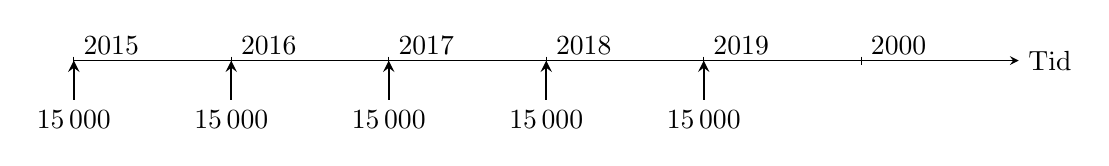
\begin{tikzpicture}[x=2cm,y=0.5cm,>=stealth]
  % Tidslinje
  \draw[->] (0,0) -- (6,0) node[right]{Tid};

  % Årstall
  \foreach \x \aar in {0/2015,1/2016,2/2017,3/2018,4/2019, 5/2000} {
    \draw (\x,0.1) -- (\x,-0.1) node[above right]{\aar};
  }
  % Innskudd
  \foreach \x in {0,1,2,3,4} {
    \draw[<-, thick] (\x,0) -- (\x,-1) node[below]{15\,000};
  }
\end{tikzpicture}
\end{center}

\end{frame}

\begin{frame}[t]{Eksempel: Hvor mye står på kontoen like etter siste innskudd}
\begin{center}
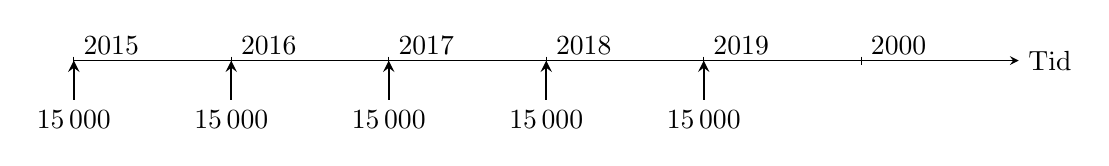
\begin{tikzpicture}[x=2cm,y=0.5cm,>=stealth]
  % Tidslinje
  \draw[->] (0,0) -- (6,0) node[right]{Tid};

  % Årstall
  \foreach \x \aar in {0/2015,1/2016,2/2017,3/2018,4/2019,5/2000} {
    \draw (\x,0.1) -- (\x,-0.1) node[above right]{\aar};
  }
  % Innskudd
  \foreach \x in {0,1,2,3,4} {
    \draw[<-, thick] (\x,0) -- (\x,-1) node[below]{15\,000};
  }
\end{tikzpicture}
\end{center}
\begin{columns}[T,onlytextwidth]
  \begin{column}{0.80\textwidth}
  \end{column}
   \begin{column}{0.20\textwidth}
    \begin{align*}
      &15\,000\cdot 1,034^0\\
      &15\,000\cdot 1,034^1\\
      &15\,000\cdot 1,034^2\\
      &15\,000\cdot 1,034^3\\
      &15\,000\cdot 1,034^4
    \end{align*}
\end{column}
\end{columns}
\end{frame}


\begin{frame}[t]{Eksempel: Hvor mye står på kontoen like etter siste innskudd}
\begin{center}
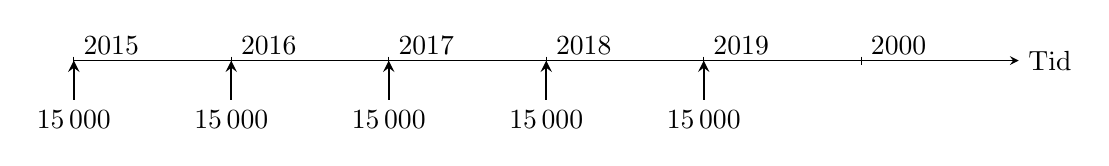
\begin{tikzpicture}[x=2cm,y=0.5cm,>=stealth]
  % Tidslinje
  \draw[->] (0,0) -- (6,0) node[right]{Tid};
  % Årstall
  \foreach \x \aar in {0/2015,1/2016,2/2017,3/2018,4/2019, 5/2000} {
    \draw (\x,0.1) -- (\x,-0.1) node[above right]{\aar};
  }
  % Innskudd
  \foreach \x in {0,1,2,3,4} {
    \draw[<-, thick] (\x,0) -- (\x,-1) node[below]{15\,000};
  }
\end{tikzpicture}
\end{center}
\begin{columns}[T,onlytextwidth]
  \begin{column}{0.80\textwidth}
  \begin{flalign*}
      &&\\
      &&\\
      &&\\
     s&=\sum_{n=1}^5 15\;000\cdot 1.034^{5-1}&\\
      &=15\;000\cdot \frac{1,034^5-1}{1,034-1}&\\
      &=80\;276,37
  \end{flalign*}
  \end{column}
   \begin{column}{0.20\textwidth}
    \begin{align*}
      &15\,000\cdot 1,034^0\\
      &15\,000\cdot 1,034^1\\
      &15\,000\cdot 1,034^2\\
      &15\,000\cdot 1,034^3\\
      &15\,000\cdot 1,034^4
    \end{align*}
\end{column}
\end{columns}
\end{frame}


\begin{comment}
\greenheader
\begin{frame}[fragile]{Eksempel: Hvor mye står på kontoen like etter siste innskudd?}

\begin{minted}[fontsize=\large]{python}
n = 5      # Antall inskudd
p = 1.034  # Rente per år
I = 15_000 # Årlig innskudd

# Første innskudd er 1. jauar 2015
# Siste innskudd er 1. januar 2019

# Bruker "list comprehension" for å lage talfølgen, minListe
minListe = [round(I*p**i) for i in range(n)]

print("Tallfølgen: ", minListe) 
# Output -> [15000, 15510, 16037, 16583, 17146]

print("Summen:", sum(minListe)) 
# Output -> Summen: 80276
\end{minted}
\end{frame}
\end{comment}

\begin{frame}[t]{Eksempel: Hvor mye står på kontoen 31. desember 2019?}
\begin{center}
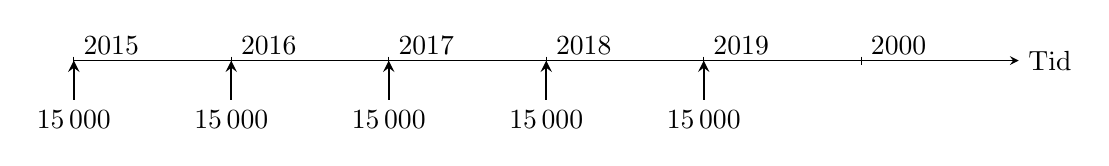
\begin{tikzpicture}[x=2cm,y=0.5cm,>=stealth]
  % Tidslinje
  \draw[->] (0,0) -- (6,0) node[right]{Tid};
  % Årstall
  \foreach \x \aar in {0/2015,1/2016,2/2017,3/2018,4/2019, 5/2000} {
    \draw (\x,0.1) -- (\x,-0.1) node[above right]{\aar};
  }
  % Innskudd
  \foreach \x in {0,1,2,3,4} {
    \draw[<-, thick] (\x,0) -- (\x,-1) node[below]{15\,000};
  }
\end{tikzpicture}
\end{center}
\begin{columns}[T,onlytextwidth]
  \begin{column}{0.80\textwidth}
  \begin{flalign*}
      &&\\
      &&\\
      &&\\
     s&=\sum_{n=1}^5 15\;000\cdot 1.034\cdot  1.034^{5-1}&\\
      &=15\;000\cdot1,034\cdot \frac{1,034^5-1}{1,034-1}&\\
      &=83\;005,76
  \end{flalign*}
  \end{column}
   \begin{column}{0.20\textwidth}
    \begin{align*}
      &15\,000\cdot 1,034^1\\
      &15\,000\cdot 1,034^2\\
      &15\,000\cdot 1,034^3\\
      &15\,000\cdot 1,034^4\\
      &15\,000\cdot 1,034^5
    \end{align*}
\end{column}
\end{columns}
\end{frame}


\begin{comment}
\greenheader
\begin{frame}[fragile]{Eksempel: Hvor mye står på kontoen 31. desember 2019?}
\begin{minted}[fontsize=\normalsize]{python}
n = 5      # Antall inskudd
p = 1.034  # Rente per år
I = 15_000 # Årlig innskudd

# Første inskudd er 1. jauar 2015
# Siste inskudd er 1. januar 2019

# Følge der første ledd er 15_000*1.034
minListe = [I*p*p**i for i in range(n)] 

print("Summen:", sum(minListe)) 
# Output -> Summen: 83005.76435177136

\end{minted}
\end{frame}
\end{comment}


\begin{frame}[t]{Eksempel: Hvor mye står på kontoen like etter siste innskudd?}
\begin{center}
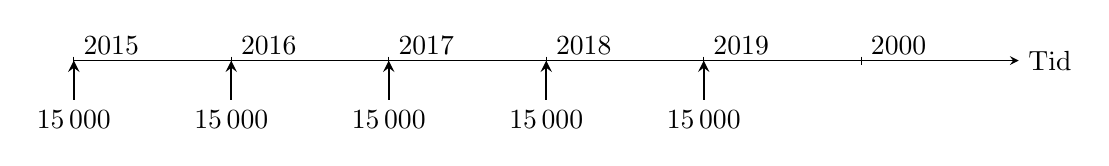
\begin{tikzpicture}[x=2cm,y=0.5cm,>=stealth]
  % Tidslinje
  \draw[->] (0,0) -- (6,0) node[right]{Tid};

  % Årstall
  \foreach \x \aar in {0/2015,1/2016,2/2017,3/2018,4/2019,5/2000} {
    \draw (\x,0.1) -- (\x,-0.1) node[above right]{\aar};
  }
  % Innskudd
  \foreach \x in {0,1,2,3,4} {
    \draw[<-, thick] (\x,0) -- (\x,-1) node[below]{15\,000};
  }
\end{tikzpicture}
\end{center}
\begin{columns}[T,onlytextwidth]
  \begin{column}{0.10\textwidth}
    \begin{align*}
      &15\,000 / 1,034^0\\
      &15\,000 / 1,034^1\\
      &15\,000 / 1,034^2\\
      &15\,000 / 1,034^3\\
      &15\,000 / 1,034^4
    \end{align*}
  \end{column}
   \begin{column}{0.90\textwidth}
\end{column}
\end{columns}
\end{frame}

\begin{frame}[t]{Eksempel: Hvor mye står på kontoen like etter siste innskudd?}
\begin{center}
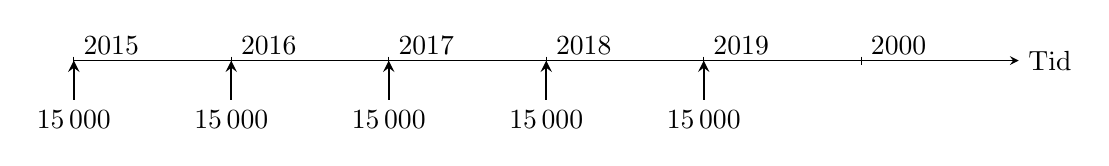
\begin{tikzpicture}[x=2cm,y=0.5cm,>=stealth]
  % Tidslinje
  \draw[->] (0,0) -- (6,0) node[right]{Tid};

  % Årstall
  \foreach \x \aar in {0/2015,1/2016,2/2017,3/2018,4/2019,5/2000} {
    \draw (\x,0.1) -- (\x,-0.1) node[above right]{\aar};
  }
  % Innskudd
  \foreach \x in {0,1,2,3,4} {
    \draw[<-, thick] (\x,0) -- (\x,-1) node[below]{15\,000};
  }
\end{tikzpicture}
\end{center}
\begin{columns}[T,onlytextwidth]
  \begin{column}{0.10\textwidth}
    \begin{align*}
      &15\,000 / 1,034^0\\
      &15\,000 / 1,034^1\\
      &15\,000 / 1,034^2\\
      &15\,000 / 1,034^3\\
      &15\,000 / 1,034^4
    \end{align*}
  \end{column}
  \begin{column}{0.30\textwidth}
  \end{column}
   \begin{column}{0.60\textwidth}
   \begin{align*}
     S_{2015}&=\sum_{n=1}^5 15\;000\cdot \left(\frac{1}{1.034}\right)^{5-1}\\
             &=15\;000\cdot \frac{\left(\frac{1}{1.034}\right)^5-1}{\frac{1}{1.034}-1}\\
             &=70\;227,23\\
     S_{2019}&=70\;227,23\cdot 1.034^4\\
             &=80\;276,37
   \end{align*}
\end{column}
\end{columns}
\end{frame}

\begin{frame}[t]{Eksempel: Hvor mye står på kontoen 31. desember 2019?}
\begin{center}
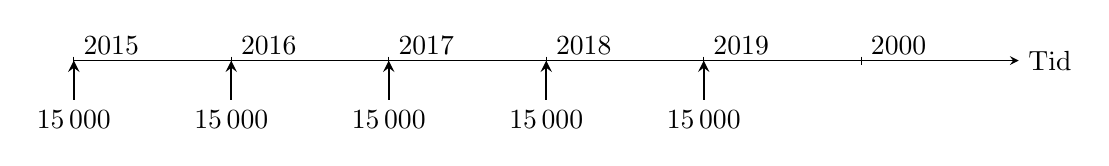
\begin{tikzpicture}[x=2cm,y=0.5cm,>=stealth]
  % Tidslinje
  \draw[->] (0,0) -- (6,0) node[right]{Tid};

  % Årstall
  \foreach \x \aar in {0/2015,1/2016,2/2017,3/2018,4/2019,5/2000} {
    \draw (\x,0.1) -- (\x,-0.1) node[above right]{\aar};
  }
  % Innskudd
  \foreach \x in {0,1,2,3,4} {
    \draw[<-, thick] (\x,0) -- (\x,-1) node[below]{15\,000};
  }
\end{tikzpicture}
\end{center}
\begin{columns}[T,onlytextwidth]
  \begin{column}{0.10\textwidth}
    \begin{align*}
      &15\,000 / 1,034^0\\
      &15\,000 / 1,034^1\\
      &15\,000 / 1,034^2\\
      &15\,000 / 1,034^3\\
      &15\,000 / 1,034^4
    \end{align*}
  \end{column}
  \begin{column}{0.30\textwidth}
  \end{column}
   \begin{column}{0.60\textwidth}
   \begin{align*}
     S_{2015}&=\sum_{n=1}^5 15\;000\cdot \left(\frac{1}{1.034}\right)^{5-1}\\
             &=15\;000\cdot \frac{\left(\frac{1}{1.034}\right)^5-1}{\frac{1}{1.034}-1}\\
             &=70\;227,23\\
     S_{2019}&==70\;227,23\cdot 1.034^5\\
             &=83\;005,76
   \end{align*}
\end{column}
\end{columns}
\end{frame}


\begin{comment}
\greenheader
\begin{frame}[fragile]{1E: Eksempel: Hvor mye står på kontoen 31. desember 2019?}
\begin{minted}[fontsize=\normalsize]{python}
n = 5      # Antall inskudd
p = 1.034  # Rente per år
I = 15_000 # Årlig innskudd

# Første inskudd er 1. jauar 2015
# Siste inskudd er 1. januar 2019

# Følge av nåverdier, første ledd er 15_000
nåverdierListe = [I/(p**i) for i in range(n)]

# Multipliserer summen med p**(n-1)
print("Summen:", sum(nåverdierListe)*p**(n-1))
# Output -> Summen: 80276.36784504
  
\end{minted}
\end{frame}
\end{comment}

\greenheader
\begin{frame}[t]{Eksempel: Annuitetslån}
\begin{center}
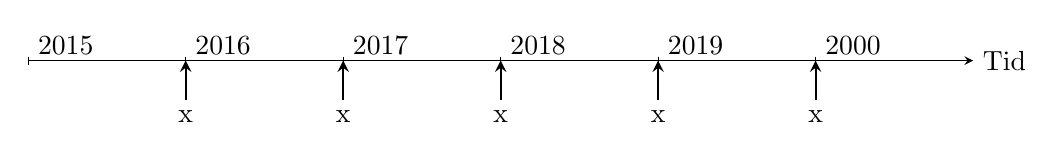
\begin{tikzpicture}[x=2cm,y=0.5cm,>=stealth]
  % Tidslinje
  \draw[->] (0,0) -- (6,0) node[right]{Tid};

  % Årstall
  \foreach \x \aar in {0/2015,1/2016,2/2017,3/2018,4/2019,5/2000} {
    \draw (\x,0.1) -- (\x,-0.1) node[above right]{\aar};
  }
  % Innskudd
  \foreach \x in {1,2,3,4,5} {
    \draw[<-, thick] (\x,0) -- (\x,-1) node[below]{x};
  }
\end{tikzpicture}
\end{center}
\medskip
\begin{itemize}
    \item Lånebeløp: $L=20\;000$ i januar 2015.\\
    \item Siste terminbeløp betales inn 31. desember 2019.
    \item Årlig rente: 7,4 \%. Vi setter $p=1,074$. 
    \item Årlig terminbeløp = $x$.
    \item Antall terminbeløp: 5.
\end{itemize}

\medskip
\textbf{Oppgave:} Finn størrelsen på det årlige terminbeløpet, $x$. 
\end{frame}

\greenheader
\begin{frame}[t]{Eksempel: Annuitetslån med sluttverdier}
\begin{center}
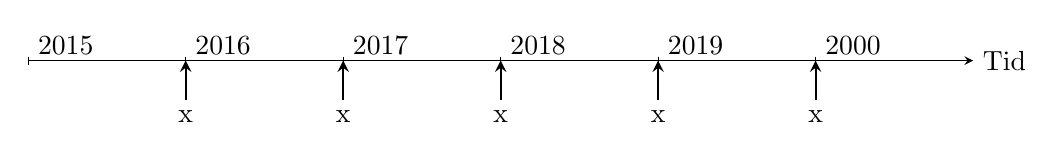
\begin{tikzpicture}[x=2cm,y=0.5cm,>=stealth]
  % Tidslinje
  \draw[->] (0,0) -- (6,0) node[right]{Tid};

  % Årstall
  \foreach \x \aar in {0/2015,1/2016,2/2017,3/2018,4/2019,5/2000} {
    \draw (\x,0.1) -- (\x,-0.1) node[above right]{\aar};
  }
  % Innskudd
  \foreach \x in {1,2,3,4,5} {
    \draw[<-, thick] (\x,0) -- (\x,-1) node[below]{x};
  }
\end{tikzpicture}
\end{center}
\begin{columns}[T,onlytextwidth]
  \begin{column}{0.50\textwidth}
  \begin{flalign*}
  &\\
  &\\
  &\\
      \sum_{n=1}^5 x\cdot 1.074^{n-1}&=20\;000\cdot 1.074^5\\
      x\cdot \frac{1,074^5-1}{1,074-1}&=20\;000\cdot 1.074^5\\
  \end{flalign*}
  \end{column}
  \begin{column}{0.20\textwidth}
  \end{column}
   \begin{column}{0.30\textwidth}
    \begin{align*}
      &x\cdot 1,074^0\\
      +\;&x\cdot 1,074^1\\
      +\;&x\cdot 1,074^2\\
      +\;&x\cdot 1,074^3\\
     +\;&x\cdot 1,074^4\\
      =\;&20\;000\cdot 1.074^5
    \end{align*}
\end{column}
\end{columns}
\end{frame}

\greenheader
\begin{frame}[t]{Eksempel: Annuitetslån med sluttverdier}
\begin{center}
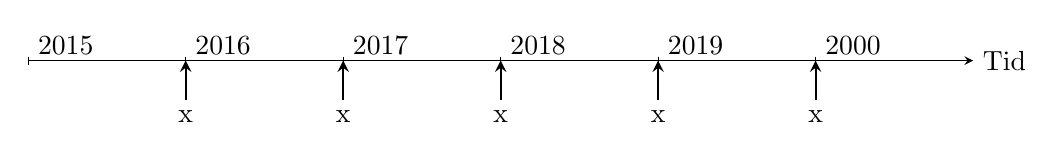
\begin{tikzpicture}[x=2cm,y=0.5cm,>=stealth]
  % Tidslinje
  \draw[->] (0,0) -- (6,0) node[right]{Tid};

  % Årstall
  \foreach \x \aar in {0/2015,1/2016,2/2017,3/2018,4/2019,5/2000} {
    \draw (\x,0.1) -- (\x,-0.1) node[above right]{\aar};
  }
  % Innskudd
  \foreach \x in {1,2,3,4,5} {
    \draw[<-, thick] (\x,0) -- (\x,-1) node[below]{x};
  }
\end{tikzpicture}
\end{center}
\begin{columns}[T,onlytextwidth]
  \begin{column}{0.70\textwidth}
 \begin{figure}
      \centering
      \includegraphics[width=0.8\linewidth]{R2K1E-1.png}
  \end{figure}
  \end{column}
   \begin{column}{0.30\textwidth}
    \begin{align*}
      &x\cdot 1,074^0\\
      +\;&x\cdot 1,074^1\\
      +\;&x\cdot 1,074^2\\
      +\;&x\cdot 1,074^3\\
     +\;&x\cdot 1,074^4\\
      =\;&20\;000\cdot 1.074^5
    \end{align*}
\end{column}
\end{columns}
\end{frame}

\greenheader
\begin{frame}[t]{Eksempel: Annuitetslån med nåverdier}
\begin{center}
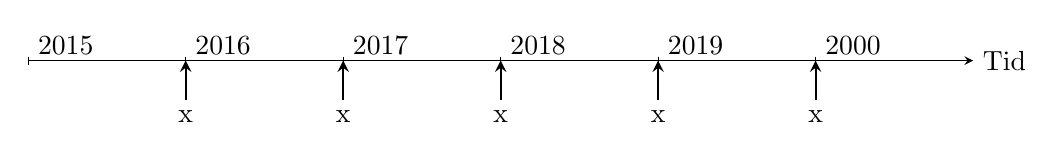
\begin{tikzpicture}[x=2cm,y=0.5cm,>=stealth]
  % Tidslinje
  \draw[->] (0,0) -- (6,0) node[right]{Tid};

  % Årstall
  \foreach \x \aar in {0/2015,1/2016,2/2017,3/2018,4/2019,5/2000} {
    \draw (\x,0.1) -- (\x,-0.1) node[above right]{\aar};
  }
  % Innskudd
  \foreach \x in {1,2,3,4,5} {
    \draw[<-, thick] (\x,0) -- (\x,-1) node[below]{x};
  }
\end{tikzpicture}
\end{center}
\begin{columns}[T,onlytextwidth]
\begin{column}{0.20\textwidth}
 \begin{align*}
      &x/ 1,074^1\\
      +\;&x/1,074^2\\
      +\;&x/ 1,074^3\\
      +\;&x/ 1,074^4\\
     +\;&x/ 1,074^5\\
      =\;&20\;000
    \end{align*}
  \end{column}
  \begin{column}{0.30\textwidth}
\end{column}
\begin{column}{0.50\textwidth}
\begin{flalign*}
  &\\
  &\\
      \sum_{n=1}^5 \frac{x}{1.074}\cdot \left(\frac{1}{1.074}\right)^{n-1}&=20\;000\\
      x\cdot \frac{\left(\frac{1}{1,074}\right)^5-1}{\frac{1}{1,074}-1}&=20\;000\\
  \end{flalign*}
\end{column}
\end{columns}
\end{frame}

\greenheader
\begin{frame}[t]{Eksempel: Annuitetslån med nåverdier}
\begin{center}
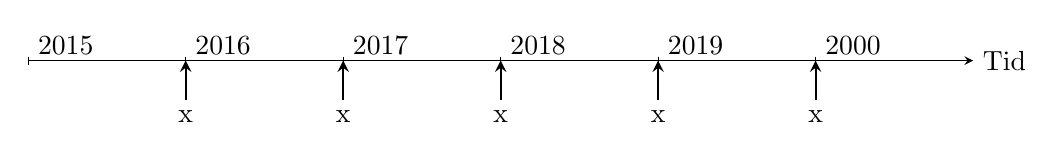
\begin{tikzpicture}[x=2cm,y=0.5cm,>=stealth]
  % Tidslinje
  \draw[->] (0,0) -- (6,0) node[right]{Tid};

  % Årstall
  \foreach \x \aar in {0/2015,1/2016,2/2017,3/2018,4/2019,5/2000} {
    \draw (\x,0.1) -- (\x,-0.1) node[above right]{\aar};
  }
  % Innskudd
  \foreach \x in {1,2,3,4,5} {
    \draw[<-, thick] (\x,0) -- (\x,-1) node[below]{x};
  }
\end{tikzpicture}
\end{center}
\begin{columns}[T,onlytextwidth]
\begin{column}{0.20\textwidth}
 \begin{align*}
      &x/ 1,074^1\\
      +\;&x/1,074^2\\
      +\;&x/ 1,074^3\\
      +\;&x/ 1,074^4\\
     +\;&x/ 1,074^5\\
      =\;&20\;000
    \end{align*}
  \end{column}
\begin{column}{0.80\textwidth}
\begin{figure}
    \centering
    \includegraphics[width=0.7\linewidth]{R2K1E-2.png}
\end{figure}
\end{column}
\end{columns}
\end{frame}






%\blueheader
%\begin{frame}{2A: Snille funksjoner kan stykkevis tilnærmes med rette %linjer}
%\begin{figure}
%    \centering
%    \includegraphics[width=0.8\linewidth]{R2-K2A-3.png}
%\end{figure}
%\end{frame}

\blueheader
\begin{frame}{2A: Det bestemte integralet}
\begin{figure}
    \centering
    \includegraphics[width=\linewidth]{R2-K2A-1.png}
\end{figure}
\end{frame}

\blueheader
\begin{frame}{2A: Nedre trappesum, $N$}
\begin{figure}
    \centering
    \includegraphics[width=0.7\linewidth]{R2-K2A-6.png}
\end{figure}

\href{https://www.geogebra.org/classic/rp6mbmm6}{Link til GeoGerba-fil}
\end{frame}

\blueheader
\begin{frame}{2A: Øvre trappesum, Ø}
\begin{figure}
    \centering
    \includegraphics[width=0.7\linewidth]{R2-K2A-7.png}

\end{figure}

\href{https://www.geogebra.org/classic/rp6mbmm6}{Link til GeoGerba-fil}
\end{frame}

\blueheader
\begin{frame}{2A: Arealet må ligge mellom nedre og øvre trappesum. $N\leq A\leq$ Ø}
\begin{figure}
    \centering
    \includegraphics[width=0.7\linewidth]{R2-K2A-8.png}

\end{figure}

\href{https://www.geogebra.org/classic/rp6mbmm6}{Link til GeoGerba-fil}
\end{frame}

\blueheader
\begin{frame}{2A: Det bestemte integralet}

La  $\{N_n\}$ være tallfølgen av nedre trappesummer.

\medskip
La  $\{\text{Ø}_n\}$ være tallfølgen av nedre trappesummer  .

\medskip
Ideen bak definisjonen av det bestemte integralet, er at trappesummene blir bedre og bedre tilnærminger for arealet når antall rektangler går mot uendelig.

\begin{blue*}{Definisjonen av det bestemte integralet}
Det bestemte integralet som en grenseverdi til en følge av summer
\begin{equation*}
    \lim_{n\rightarrow \infty }N_ n =\lim_{n\rightarrow \infty }\text{Ø}_n=\int_a^bf(x)\;dx
\end{equation*}
Dersom grenseverdiene er forskjellige, er $f$ ikke integrerbar.
\end{blue*}
\end{frame}

\redheader
\begin{frame}{2A: Integrerbare funksjoner}
Hvis $f$ er en \textbf{kontinuerlig funksjon} på et intervall $[a,b]$ på x-aksen,  
så kan vi alltid regne ut \textbf{integralet} av $f$ på dette intervallet.  

\medskip

\[
    \int_a^b f(x)\,dx
\]

\medskip
\begin{itemize}
    \item Integral = ''arealet'' mellom grafen til $f$  
          og x-aksen i intervallet fra $x=a$ til $x=b$.
    \item ''Areal'' over x-aksen er positivt, og ''arealet'' under x-aksen er negativt.
\end{itemize}
\end{frame}

\blueheader
\begin{frame}[fragile]{2A: Integraler i GeoGebra: \texttt{integral(funksjon, start, slutt)}}
\begin{figure}
    \centering
    \includegraphics[width=\linewidth]{R2-K2A-9.png}
    \caption{\texttt{integral(0.5x-1, 0, 2)}}
\end{figure}
\end{frame}

\blueheader
\begin{frame}[fragile]{2A: Integraler i GeoGebra: \texttt{integral(funksjon, start, slutt)}}
\begin{figure}
    \centering
    \includegraphics[width=\linewidth]{R2-K2A-10.png}
    \caption{\texttt{integral(0.5x-1, 2, 4)}}
\end{figure}
\end{frame}

\blueheader
\begin{frame}[fragile]{2A: Integraler i GeoGebra: \texttt{integral(funksjon, start, slutt)}}
\begin{figure}
    \centering
    \includegraphics[width=\linewidth]{R2-K2A-11.png}
    \caption{\texttt{integral(0.5x-1, 0, 4)}}
\end{figure}
\end{frame}

\blueheader
\begin{frame}[fragile]{2A: Integraler i kombinasjon med \emph{Dersom} i CAS}
\begin{figure}
    \centering
    \includegraphics[width=\linewidth]{R2-K2A-13.png}
\end{figure}
\end{frame}

\blueheader
\begin{frame}[fragile]{2A: Integraler i kombinasjon med \emph{Løs} i CAS}
\begin{figure}
    \centering
    \includegraphics[width=\linewidth]{R2-K2A-12.png}
\end{figure}
\end{frame}

\greenheader
\begin{frame}[fragile]{2A: Integraler i Python hvis dere vil}
    \warn
\begin{figure}
    \centering
    \includegraphics[width=0.5\linewidth]{R2-K2A-14.png}
\end{figure}
\end{frame}


\greenheader
\begin{frame}{2A: Nedre trappesum, $N_n$,  for en strengt voksende funksjon}
    \begin{columns} 
        \begin{column}{0.42\textwidth}
            Bredden av rektanglene på figuren er 
            \[
                \Delta x = \frac{b-a}{n}.
            \]
            Høyden i rektanglene er 
            \[
                f(x_0), f(x_1), f(x_2), \dots, f(x_{n-1}).
            \]
           
            
        \end{column}
        \begin{column}{0.58\textwidth}
            \centering
            \includegraphics[width=1\linewidth]{R2-K2A-15.png}
        \end{column}
    \end{columns}
    \begin{align*}
                 N_n &=  
                 f(x_0)\cdot \Delta x + f(x_1)\cdot \Delta x + f(x_2)\cdot \Delta x \dots + f(x_{n-1})\cdot \Delta x\\
                &=  \sum_{i=1}^{n} f(x_{i-1})\cdot \Delta x
            \end{align*}
\end{frame}

\greenheader
\begin{frame}{2A: Øvre trappesum $\text{Ø}_n$,  for en strengt voksende funksjon}
    \begin{columns} 
        \begin{column}{0.42\textwidth}
            Bredden av rektanglene på figuren er 
            \[
                \Delta x = \frac{b-a}{n}.
            \]
            Høyden i rektanglene er 
            \[
                f(x_1), f(x_2), f(x_3), \dots, f(x_{n}).
            \]
           
            
        \end{column}
        \begin{column}{0.58\textwidth}
            \centering
            \includegraphics[width=1\linewidth]{R2-K2A-15.png}
        \end{column}
    \end{columns}
    \begin{align*}
                 \text{Ø}_n &=  
                 f(x_1)\cdot \Delta x + f(x_2)\cdot \Delta x + f(x_3)\cdot \Delta x \dots + f(x_{n})\cdot \Delta x\\
                &=  \sum_{i=1}^{n} f(x_{i})\cdot \Delta x
            \end{align*}
\end{frame}

\blueheader
\begin{frame}{2B: Nedre trappesum til en ikke er strengt voksende funksjon}
Merk at generelt tar 
\begin{itemize}
    \item nedre trappesum utgangspunkt i den minste høyden til rektanglet.\\
    \item og øvre trappesum tar utgangspunkt i den største høyden til rektanglet.
\end{itemize}
\begin{figure}
    \centering
    \includegraphics[width=0.6\linewidth]{R2-K2A-17.png}
\end{figure}
\end{frame}

\blueheader
\begin{frame}{2B: Venstre- og høyre-tilnærming}
\begin{figure}
    \centering
    \includegraphics[width=\linewidth]{R2-K2B-2.png}
\end{figure}
\end{frame}







\blueheader
\begin{frame}{2B: Riemannsummer. Velger en vilkårlig x-verdi, $x^*\in[x_{i-1},x_i]$}
    \begin{columns} 
        \begin{column}{0.35\textwidth}
    \textbf{Venstretilnærming:}
        \begin{equation*}
            \sum_{i=1}^n f(x_{i-1})\cdot \Delta x
        \end{equation*}
      \textbf{Høyretilnærming:}
        \begin{equation*}
            \sum_{i=1}^n f(x_{i})\cdot \Delta x
        \end{equation*}
    \textbf{Riemansum:}
       \begin{equation*}
            \sum_{i=1}^n f(x^*_{i})\cdot \Delta x
        \end{equation*}
        \end{column}
        \begin{column}{0.65\textwidth}
            \centering
            \includegraphics[width=1\linewidth]{R2-K2B-1.png}
        \end{column}
    \end{columns}
\end{frame}

\redheader
\begin{frame}{2B: Det bestemte integralet}
    Det bestemte integralet kan uttrykkes som en grenseverdi til en følge av riemannsummer.

    \begin{equation*}
        \int_a^b f(x)\;dx=\lim_{n\rightarrow\infty}\sum_{i=1}^nf(x_i^*)\cdot \Delta x, \:\;\; \text{der} \;\;\; \Delta x = \frac{b-a}{n}
    \end{equation*}
\end{frame}

\redheader
\begin{frame}{2B: Rektangelmetoden med venstretilnærming}
 \begin{equation*}
        \int_a^b f(x)\;dx=\lim_{n\rightarrow\infty}\sum_{i=1}^nf(x_{i-1})\cdot \Delta x, \:\;\; \text{der} \;\;\; x_{i-1}=a+(i-1)\cdot \Delta x
    \end{equation*}
    \begin{figure}
        \centering
   \includegraphics[width=\linewidth]{R2-K2B-2.png}
    \end{figure}
\end{frame}

\redheader
\begin{frame}{2B: Rektangelmetoden med høyretilnærming}
 \begin{equation*}
        \int_a^b f(x)\;dx=\lim_{n\rightarrow\infty}\sum_{i=1}^nf(x_{i})\cdot \Delta x, \:\;\; \text{der} \;\;\; x_{i}=a+i\cdot \Delta x
    \end{equation*}

     \begin{figure}
        \centering
   \includegraphics[width=\linewidth]{R2-K2B-2.png}
    \end{figure}
\end{frame}


\greenheader
\begin{frame}{2B: Eksempel 5 side 106 (Venstretilnærming)}
\begin{figure}
    \centering
    \includegraphics[width=\linewidth]{R2-K2B-3.png}
\end{figure}
\end{frame}

\greenheader
\begin{frame}[fragile]{2B: Eksempel 5 side 106: Venstretilnærming og høyretilnærming i python}
\begin{minted}[fontsize=\small]{python}
a, b = 1, 5               # Nedre og øvre grense i intervallet [a, b]
n = 10                    # Antall rektangler

def f(x):
  return x**2 - 2*x + 2

venstre_sum = 0           # Summen av arealene til venstre-tilnærming-rektangler
høyre_sum   = 0           # Summen av arealene til høyre-tilnærming-rektangler
delta_x = (b-a)/n         # Rektangelbredden

for i in range(1, n+1):
  venstre_sum = venstre_sum + f(a+(i-1)*delta_x)*delta_x
  høyre_sum = høyre_sum + f(a+i*delta_x)*delta_x

print(f"Venstresummen: {round(venstre_sum,2)}")     # Venstresummen: 22.24
print(f"Høyresummen: {round(høyre_sum,2)}")         # Høyresummen: 28.64
print(f"Gjennomsnitt: {(venstre_sum+høyre_sum)/2}") # Gjennomsnitt: 25.44
\end{minted}
\end{frame}

\greenheader
\begin{frame}{2B: Eksempel 6 side 108: Venstretilnærming}
Funksjonen $f$ har verditabellen
\begin{table}[h]
\centering
\begin{tabular}{c|ccccccccc}
$x$ & 0 & 0,5 & 1 & 1,5 & 2 & 2,5 & 3 & 3,5 & 4 \\
\hline
$f(x)$ & 13,1 & 16,3 & 0 & 8,2 & 19,7 & 24,8 & 28,1 & 27,3 & 21,0 \\
\end{tabular}
\end{table}
Lag et program som finner en tilnærmingsverdi for $\int_0^4 f(x)\;dx$ med en venstretilnærming.
\begin{figure}
    \centering
    \includegraphics[width=0.9\linewidth]{R2-K2B-4.png}

\end{figure}
\end{frame}

\greenheader
\begin{frame}[fragile]{2B: Eksempel 6 side 108: Venstretilnærming}
\begin{minted}[fontsize=\small]{python}
# lister med x-verdier og funksjonsverdier
x = [0, 0.5, 1, 1.5, 2, 2.5, 3, 3.5, 4]
f = [13.1, 16.3, 0, 8.2, 19.7, 24.8, 28.1, 27.3, 21.0]

delta_x = x[1] - x[0]     # rektangelbredde
n = len(x)                # antall x-verdier i lista
summen = 0

# Legg merke til at n = len(x) = 9, og siden "i" i for-løkken 
# starter på 0, må "i" gå til n-1=8, og at maks verdi for "i" er 7.

for i in range(n-1):    
  summen = summen + f[i] * delta_x

print(round(summen, 1)) # Output: 68.8

# Legg merke til at det står f[i], og ikke f[i-1], selv om dette er en 
# venstretilnærming. Det er fordi "i" i for-løkken starter på null. 
\end{minted}
\end{frame}




\redheader
\begin{frame}{2B: Midtpunkttilnærming}
 \begin{equation*}
        \int_a^b f(x)\;dx\approx\sum_{i=1}^nf(m_{i})\cdot \Delta x, \:\;\; \text{der} \;\;\; m_{i}=a+\left(i-\frac{1}{2}\right)\cdot \Delta x
    \end{equation*}

     \begin{figure}
        \centering
   \includegraphics[width=0.7\linewidth]{R2-K2B-5.png}
    \end{figure}
\end{frame}


\greenheader
\begin{frame}{2B: Eksempel 5 side 105: Midtpunkttilnærming. Fasit: 25,33}
Funksjonen $f$ er gitt ved $f(x)=x^2-2x+2$. Lag et program som finner en tilnærmingsverdi for integralet ved å bruke midtpunkttilnærming med 10 kvadrater.
\[
\int_1^5f(x)\;dx
\].
\begin{figure}
    \centering
    \includegraphics[width=0.9\linewidth]{R2-K2B-7.png}
\end{figure}
\end{frame}


\greenheader
\begin{frame}[fragile]{2B: Eksempel 5 side 105: Midtpunkttilnærming. Fasit: 25,33}
\begin{minted}[fontsize=\small]{python}
a, b = 1, 5     # Nedre og øvre grense i intervallet [a, b]
n = 10          # Antall rektangler

def f(x):
    return x**2 - 2*x + 2

delta_x = (b - a) / n
summen = 0.0

for i in range(n):
    x_midt = a + (i + 0.5) * delta_x
    summen = summen + f(x_midt) * delta_x

print(f"Midtpunktsummen: {round(summen, 2)}") # Output: 25.28
\end{minted}
\end{frame}

\greenheader
\begin{frame}{2B: Eksempel 6 side 108: Midtpunkttilnærming}
Funksjonen $f$ har verditabellen
\begin{table}[h]
\centering
\begin{tabular}{c|ccccccccc}
$x$ & 0 & 0,5 & 1 & 1,5 & 2 & 2,5 & 3 & 3,5 & 4 \\
\hline
$f(x)$ & 13,1 & 16,3 & 0 & 8,2 & 19,7 & 24,8 & 28,1 & 27,3 & 21,0 \\
\end{tabular}
\end{table}
Lag et program som finner en tilnærmingsverdi for $\int_0^4 f(x)\;dx$ med en midtpunkttilnærming.
\begin{figure}
    \centering
    \includegraphics[width=0.8\linewidth]{R2-K2B-6.png}

\end{figure}
\end{frame}

\greenheader
\begin{frame}[fragile]{2B: Eksempel 6 side 108: Midtpunkttilnærming}
\begin{minted}[fontsize=\small]{python}
# To lister med x-verdier og funksjonsverdier
x = [0, 0.5, 1, 1.5, 2, 2.5, 3, 3.5, 4]
f = [13.1, 16.3, 0, 8.2, 19.7, 24.8, 28.1, 27.3, 21.0]

delta_x = x[1] - x[0]  # rektangelbredde
n = len(x)  # antall x-verdier i lista
summen = 0

# Midtpunktstilnærming
for i in range(n-1):
    # Bruk gjennomsnittet som approksimasjon av funksjonsverdi i midten
    midt_f = (f[i] + f[i+1]) / 2
    summen = summen + midt_f * delta_x

print(round(summen, 1))

\end{minted}
\end{frame}


\blueheader
\begin{frame}{2B: Arealformelen til et trapes}
\begin{columns}[c] % [c] = midtstill innholdet vertikalt
  \begin{column}{0.45\textwidth}
    \[
      A = \frac{h}{2}(a+b)
    \]
    \begin{itemize}
      \item \(a, b\) = parallelle sider
      \item \(h\) = høyden
    \end{itemize}

Men i vårt tilfelle er det bedre å skrive arealformelen slik:

\begin{equation*}
    A=\frac{4-2}{2}\left(f(2)+f(4)\right)
\end{equation*}

Generelt får vi (hvis \emph{i} starter på 1):
\begin{equation*}
    A=\frac{\Delta x}{2}\left(f(x_{i-1})+f(x_{i})\right)
\end{equation*}
  \end{column}
  \begin{column}{0.55\textwidth}
    \begin{figure}
      \centering
      \includegraphics[width=\linewidth]{R2-K2B-8.png}
    \end{figure}
  \end{column}
\end{columns}
\end{frame}

\redheader
\begin{frame}{2B: Trapesetoden}
 \begin{equation*}
        \int_a^b f(x)\;dx\approx\frac{\Delta x}{2}\left(f(a)+f(b)+2\cdot \sum_{i=1}^{n-1}f(x_i)\right),\;\;\;\texttt{der}\;\;\; x_i=a+i\cdot \Delta x
    \end{equation*}
     \begin{figure}
        \centering
   \includegraphics[width=0.8\linewidth]{R2-K2B-9.png}
    \end{figure}
(Beviset står på side 110)
\end{frame}


\greenheader
\begin{frame}{2B: Eksempel 5 side 105: Trapesmetoden. Fasit: 25,33}
Funksjonen $f$ er gitt ved $f(x)=x^2-2x+2$. Lag et program som finner en tilnærmingsverdi for integralet ved å bruke trapesmetoden med 10 kvadrater.
\[
\int_1^5f(x)\;dx
\].
\begin{figure}
    \centering
    \includegraphics[width=0.9\linewidth]{R2-K2B-10.png}
\end{figure}
\end{frame}


\greenheader
\begin{frame}[fragile]{2B: Eksempel 5 side 105: Trapesmetoden. Fasit: 25,33}
\begin{minted}[fontsize=\small]{python}
a, b = 1, 5   # Intervallet [a, b]
n = 10        # Antall delintervaller
delta_x = (b - a) / n
summen = 0.0

def f(x):
    return x**2 - 2*x + 2

# Bruker List comprehension til å lage lister med x- og y-verdier. 
x_liste = [a + i*delta_x for i in range(n+1)]
y_liste = [f(x) for x in x_liste]

# Trapesmetoden. Utfordring: Forklar at denne koden 
# stemmer med trapes-metode-formelen.
for i in range(n): 
    summen = summen + (y_liste[i] + y_liste[i+1]) * delta_x / 2

print(f"Trapesmetoden: {round(summen, 2)}") # Output: 25.44
\end{minted}
\end{frame}


\greenheader
\begin{frame}{2B: Eksempel 6 side 108: Trapesmetoden}
Funksjonen $f$ har verditabellen
\begin{table}[h]
\centering
\begin{tabular}{c|ccccccccc}
$x$ & 0 & 0,5 & 1 & 1,5 & 2 & 2,5 & 3 & 3,5 & 4 \\
\hline
$f(x)$ & 13,1 & 16,3 & 0 & 8,2 & 19,7 & 24,8 & 28,1 & 27,3 & 21,0 \\
\end{tabular}
\end{table}
Lag et program som finner en tilnærmingsverdi for $\int_0^4 f(x)\;dx$ med en trapesmetoden.
\begin{figure}
    \centering
    \includegraphics[width=0.8\linewidth]{R2-K2B-11.png}

\end{figure}
\end{frame}

\greenheader
\begin{frame}[fragile]{2B: Eksempel 6 side 108: Trapesmetoden}
\begin{minted}[fontsize=\normalsize]{python}
# Dataene fra tabellen
x = [0, 0.5, 1, 1.5, 2, 2.5, 3, 3.5, 4]
f = [13.1, 16.3, 0, 8.2, 19.7, 24.8, 28.1, 27.3, 21.0]

delta_x = x[1] - x[0]  # bredde
n = len(x) - 1         # antall delintervaller
summen = 0

# Trapesmetoden
for i in range(n):
    summen += (f[i] + f[i+1]) * delta_x / 2

print(f"Trapesmetoden: {round(summen, 2)}") # Output: 70.73
\end{minted}
\end{frame}






















% -----------------------
\greenheader
\begin{frame}[fragile]{2B: Generell pythonkode for å regne ut nedre trappesum  (Utfordring)}
\begin{minted}[fontsize=\small]{python} 
def f(x):
    return 0.1*x*(x-4)*(x-8)  # Funksjonen vi skal integrere tilnærmet

start, slutt = 0, 8           # Integrasjonsintervall [0, 8]
bredde = 0.1                  # Bredde på hvert rektangel
antall = round((slutt-start)/bredde)  # Antall rektangler i intervallet
N, Ø = 0, 0  # Startverdier for nedre og øvre trappesum

for i in range(antall):
    x_venstre = start + i*bredde      # Venstre endepunkt for intervallet
    x_høyre = x_venstre + bredde      # Høyre endepunkt for intervallet
    f_venstre = f(x_venstre)          # Funksjonsverdi i venstre endepunkt
    f_høyre = f(x_høyre)              # Funksjonsverdi i høyre endepunkt
    N = N + bredde * min(f_venstre, f_høyre)  # Areal med minste funksjonsverdi
    
print(f"Antall rektangler: {antall}") 
print(f"Rektangelbredde: {bredde}")
print(f"Nedre trappesum: {N}")
\end{minted}
\end{frame}


\greenheader
\begin{frame}[fragile]{2B: Generell pythonkode for å regne ut øvre trappesum  (Utfordring) }
\begin{minted}[fontsize=\small]{python}
def f(x):
    return 0.1*x*(x-4)*(x-8)  # Funksjonen vi skal integrere tilnærmet

start, slutt = 0, 8           # Integrasjonsintervall [0, 8]
bredde = 0.1                  # Bredde på hvert rektangel
antall = round((slutt-start)/bredde)  # Antall rektangler i intervallet
N, Ø = 0, 0  # Startverdier for nedre og øvre trappesum

for i in range(antall):
    x_venstre = start + i*bredde      # Venstre endepunkt for intervallet
    x_høyre = x_venstre + bredde      # Høyre endepunkt for intervallet
    f_venstre = f(x_venstre)          # Funksjonsverdi i venstre endepunkt
    f_høyre = f(x_høyre)              # Funksjonsverdi i høyre endepunkt
    Ø = Ø + bredde * max(f_venstre, f_høyre)  # Areal med største funksjonsverdi

print(f"Antall rektangler: {antall}") 
print(f"Rektangelbredde: {bredde}")
print(f"Øvre trappesum: {Ø}")
\end{minted}
\end{frame}
\redheader
\begin{frame}{2C: Tolkning av integralet}
Arealet av området mellom en graf og førsteaksen har samme enhet som produktet av enhetene på aksene
    \begin{figure}
        \centering
        \includegraphics[width=0.5\linewidth]{R2-K2C-1.png}
    \end{figure}
\end{frame}

\greenheader
\begin{frame}{2C: Eksempel 7 side 114}
Modellen beskriver hvor mange liter vann som renner ut av et akvarium per sekund.
\begin{equation*}
    V(t)=3,8\cdot e^{-0.05t} 
\end{equation*}
Arealet under grafen har enheten liter.\\

Hvor mye vann renner ut i løpet av det første minuttet? 
\begin{figure}
    \centering
    \includegraphics[width=0.8\linewidth]{R2-K2C-2.png}
\end{figure}
\end{frame}

\redheader
\begin{frame}{2C: Arealet under førsteaksen}
    La $A$ være arealet av området avgrenset av grafen til den kontinuerlige funksjonen $f$, x-aksen og linjene $x=a$ og $x=b$.\\
    \begin{align*} 
    \text{Arealet }  A&=\int_a^bf(x)\;dx \text{   hvis området ligger over x-aksen.}\\
       \text{Arealet }  A&=-\int_a^bf(x)\;dx \text{   hvis området ligger under x-aksen.}
       \end{align*}
       
    \medskip
    Hvis området ligger delvis over og delvis under x-aksen, må vi dele det opp i flere deler og summere delarealene.
\end{frame}


\greenheader\begin{frame}{2C: Eksempel 8 side 117}
\begin{figure}
    \centering
    \includegraphics[width=0.9\linewidth]{R2-K2C-3.png}
\end{figure}
\end{frame}

\greenheader\begin{frame}{2C: Eksempel 10 side 122}
\begin{figure}
    \centering
    \includegraphics[width=\linewidth]{R2-K2C-4.png}
\end{figure}
\end{frame}

\greenheader\begin{frame}{2C: Eksempel 10 side 122}
\begin{figure}
    \centering
    \includegraphics[width=\linewidth]{R2-K2C-5.png}
\end{figure}
\end{frame}

\redheader
\begin{frame}{2C: Arealet mellom to grafer}
    \begin{columns}
        \begin{column}{0.3\linewidth}
            \begin{figure}
                \centering
                \includegraphics[width=\linewidth]{R2-K2B-12.png}
            \end{figure}
        \end{column}
        \begin{column}{0.6\linewidth}
            Hvis \(f(x)\geq g(x)\) for alle \(x\) i \([a,b]\), er arealet av området mellom grafene til \(f\) og \(g\), og linjene \(x=a\) og \(x=b\) gitt ved
            \begin{equation*}
                A = \int_a^b (f(x) - g(x)) \;dx
            \end{equation*}
        \end{column}
    \end{columns}
\end{frame}

\greenheader\begin{frame}{2C: Eksempel 10 side 122}
\begin{figure}
    \centering
    \includegraphics[width=\linewidth]{R2-K2C-7.png}
\end{figure}
\end{frame}

\greenheader
\begin{frame}[fragile]{2C: Areal mellom funksjonene f og g i python (hvis dere vil)}
\begin{minted}[fontsize=\footnotesize]{python}
from pylab import *

def f(x):
  return (x+4)**0.5      # f(x) = kvadratroten av (x+4)

def g(x):
  return x**2 - 1        # g(x) = x^2 - 1

# Skjæringspunktene mellom f og g (løst på forhånd)
a = -1.5969  # Nedre grense
b =  1.8489  # Øvre grense

# Lager en liste med 100 jevnt fordelte x-verdier mellom a og b
x = linspace(a, b, 100)

# Arealet mellom f og g finner vi ved å integrere (f(x) - g(x))
# Her bruker vi trapesmetoden (numerisk tilnærming)
svar = trapezoid(f(x) - g(x), x)
print(svar) # Oputput: 6.927568467295032
\end{minted}
\end{frame}


\redheader
\begin{frame}{2C: Gjennomsnittsverdiern til en funksjon i intervallet $[a, b]$}
Gjennomsnittsverdien til en kontinuerlig funksjon \(f\) i intervallet \([a,b]\) er gitt ved
\[\text{Gjennomsnittsverdi} = \frac{1}{b-a}\int_a^b f(x) \; dx.\]
\begin{figure}
    \centering
    \includegraphics[width=0.6\linewidth]{R2-K2B-13.png}
\end{figure}    
\end{frame}

\greenheader
\begin{frame}{2C: Oppgave 2.51 side 126}
    På en fabrikk der det skilles ut et skadelig stoff, ble konsentrasjonen av stoffet målt gjennom en hel arbeidsdag.\(K(t)\) er konsentrasjonen ved tidspunktet \(t\). Arbeidsmiljøloven krever at den gjennomsnittlige konsentrasjonen i løpet av arbeidsdagen ikke overstiger \(140\,\mathrm{mg}/\mathrm{m}^3\). Var kravet i arbeidsmiljøloven oppfylt denne dagen?

\begin{figure}
    \centering
    \includegraphics[width=0.6\linewidth]{R2-K2B-13.png}
\end{figure}
\end{frame}

\magentaheader
\begin{frame}{2C: Buelengde til en graf i \([a, b]\) (Utforsk side 126)}
    \begin{columns}
        \begin{column}{0.40\linewidth}
            Lengden av grafen til \(f\) i intervallet \([a, b]\) kan tilnærmes ved å summere små linjestykker:
            \[
            s_i \approx \sqrt{(\Delta x)^2 + (f(x_{i+1}) - f(x_i))^2}
            \]
            Den eksakte buelengden er gitt ved
            \[
            s = \int_a^b \sqrt{1 + (f'(x))^2} \; dx
            \]
        \end{column}
        \begin{column}{0.60\linewidth}
            \begin{figure}
                \centering
                \includegraphics[width=\linewidth]{R2-K2C-8.png}
            \end{figure}
        \end{column}
    \end{columns}
\end{frame}


\greenheader
\begin{frame}{2C: Buelengden til en halvsirkel}
\begin{figure}
    \centering
    \includegraphics[width=1\linewidth]{R2K1C-4.png}
\end{figure}
\end{frame}

\blueheader
\begin{frame}{2D: Snille funksjoner kan stykkevis tilnærmes med rette linjer}
\begin{figure}
    \centering
    \includegraphics[width=0.8\linewidth]{R2-K2A-3.png}
\end{figure}
\end{frame}

% Første frame
\blueheader
\begin{frame}{2D: Ideen som forbinder integralet med den deriverte}
\begin{columns}[onlytextwidth]
  \begin{column}{0.45\textwidth}
    La \(A(x)\) være arealet mellom grafen til \(f\)  og x-aksen fra \(0\) til \(x\):
    \[
    A(x)=\int_{0}^{x} f(t)\,dt.
    \]

    For en liten økning \(\Delta x\) er arealet fra \(x\) til \(x+\Delta x\) omtrent lik $ f(x)\cdot\Delta x$
    \begin{align*}
      A(x+\Delta x)-A(x) &\approx f(x)\,\Delta x\\[0.8em]
      \frac{A(x+\Delta x)-A(x)}{\Delta x} &\approx f(x)\\[0.8em]
      A'(x) &\approx f(x)
    \end{align*}
  \end{column}
  \begin{column}{0.55\textwidth}
    \centering
    \includegraphics[width=\linewidth]{R2-K2A-4.png}
  \end{column}
\end{columns}
\end{frame}

% Andre frame
\greenheader
\begin{frame}{2D: Sammenhengen mellom posisjon og fart}
\begin{columns}[T,onlytextwidth]
   \begin{column}{0.45\textwidth}
    \begin{align*}
      s(t+\Delta t)-s(t) &\approx v(t)\,\Delta t\\[0.8em]
      \frac{s(t+\Delta t)-s(t)}{\Delta t} &\approx v(t)\\[0.8em]
      s'(t) &\approx v(t)
    \end{align*}
  \end{column}
   \begin{column}{0.55\textwidth}
    \centering
    \includegraphics[width=\linewidth]{R2-K2A-5.png}
  \end{column}
\end{columns}
\end{frame}



\end{document}
